\documentclass[12pt,a4paper,titlepage]{scrartcl}

\usepackage{comment}
\usepackage[main=english]{babel}
\usepackage[utf8]{inputenc}
\usepackage[T1]{fontenc}
\usepackage{lmodern}
\usepackage{geometry}
\geometry{left=2.5cm,right=2.5cm,top=2.5cm,bottom=3cm,head=29pt,foot=25pt}
\setlength{\footheight}{25pt}
\usepackage{microtype}
\usepackage{amsmath,amssymb,mathtools}
\numberwithin{equation}{section}
\numberwithin{table}{section}
\numberwithin{figure}{section}
\usepackage{siunitx}
\sisetup{locale=US, separate-uncertainty=true, per-mode=fraction}
\usepackage{booktabs}
\usepackage{multirow}
\usepackage{graphicx}
\usepackage{float}
\usepackage{caption}
\usepackage{subcaption}
\usepackage[automark]{scrlayer-scrpage}
\usepackage[most]{tcolorbox}
\usepackage{hyperref}
\usepackage{pdfpages}
\usepackage{csvsimple-l3}
\usepackage{longtable}
\usepackage{graphicx}


% Basic figure setup, for now with no caption control since it's done
% automatically by Pandoc (which extracts ![](path) syntax from Markdown).
\usepackage{graphicx}
% Keep aspect ratio if custom image width or height is specified
\setkeys{Gin}{keepaspectratio}
% Maintain compatibility with old templates. Remove in nbconvert 6.0
\let\Oldincludegraphics\includegraphics
\usepackage{caption}

\usepackage{float}

\floatplacement{figure}{H} % forces figures to be placed at the correct location
\usepackage{xcolor} % Allow colors to be defined
\usepackage{enumerate} % Needed for markdown enumerations to work
\usepackage{geometry} % Used to adjust the document margins
\usepackage{amsmath} % Equations
\usepackage{amssymb} % Equations
\usepackage{textcomp} % defines textquotesingle
% Hack from http://tex.stackexchange.com/a/47451/13684:
\AtBeginDocument{%
    \def\PYZsq{\textquotesingle}% Upright quotes in Pygmentized code
}
\usepackage{upquote} % Upright quotes for verbatim code
\usepackage{eurosym} % defines \euro

\usepackage{iftex}
\ifPDFTeX
    \usepackage[T1]{fontenc}
    \IfFileExists{alphabeta.sty}{
            \usepackage{alphabeta}
        }{
            \usepackage[mathletters]{ucs}
            \usepackage[utf8x]{inputenc}
        }
\else
    \usepackage{fontspec}
    \usepackage{unicode-math}
\fi

\usepackage{fancyvrb} % verbatim replacement that allows latex
\usepackage{grffile} % extends the file name processing of package graphics
                        % to support a larger range
\makeatletter % fix for old versions of grffile with XeLaTeX
\@ifpackagelater{grffile}{2019/11/01}
{
    % Do nothing on new versions
}
{
    \def\Gread@@xetex#1{%
    \IfFileExists{"\Gin@base".bb}%
    {\Gread@eps{\Gin@base.bb}}%
    {\Gread@@xetex@aux#1}%
    }
}
\makeatother
\usepackage[Export]{adjustbox} % Used to constrain images to a maximum size
\adjustboxset{max size={0.9\linewidth}{0.9\paperheight}}

% The hyperref package gives us a pdf with properly built
% internal navigation ('pdf bookmarks' for the table of contents,
% internal cross-reference links, web links for URLs, etc.)
\usepackage{hyperref}
% The default LaTeX title has an obnoxious amount of whitespace. By default,
% titling removes some of it. It also provides customization options.
\usepackage{titling}
\usepackage{longtable} % longtable support required by pandoc >1.10
\usepackage{booktabs}  % table support for pandoc > 1.12.2
\usepackage{array}     % table support for pandoc >= 2.11.3
\usepackage{calc}      % table minipage width calculation for pandoc >= 2.11.1
\usepackage[inline]{enumitem} % IRkernel/repr support (it uses the enumerate* environment)
\usepackage[normalem]{ulem} % ulem is needed to support strikethroughs (\sout)
                            % normalem makes italics be italics, not underlines
\usepackage{soul}      % strikethrough (\st) support for pandoc >= 3.0.0
\usepackage{mathrsfs}



% Colors for the hyperref package
\definecolor{urlcolor}{rgb}{0,.145,.698}
\definecolor{linkcolor}{rgb}{.71,0.21,0.01}
\definecolor{citecolor}{rgb}{.12,.54,.11}

% ANSI colors
\definecolor{ansi-black}{HTML}{3E424D}
\definecolor{ansi-black-intense}{HTML}{282C36}
\definecolor{ansi-red}{HTML}{E75C58}
\definecolor{ansi-red-intense}{HTML}{B22B31}
\definecolor{ansi-green}{HTML}{00A250}
\definecolor{ansi-green-intense}{HTML}{007427}
\definecolor{ansi-yellow}{HTML}{DDB62B}
\definecolor{ansi-yellow-intense}{HTML}{B27D12}
\definecolor{ansi-blue}{HTML}{208FFB}
\definecolor{ansi-blue-intense}{HTML}{0065CA}
\definecolor{ansi-magenta}{HTML}{D160C4}
\definecolor{ansi-magenta-intense}{HTML}{A03196}
\definecolor{ansi-cyan}{HTML}{60C6C8}
\definecolor{ansi-cyan-intense}{HTML}{258F8F}
\definecolor{ansi-white}{HTML}{C5C1B4}
\definecolor{ansi-white-intense}{HTML}{A1A6B2}
\definecolor{ansi-default-inverse-fg}{HTML}{FFFFFF}
\definecolor{ansi-default-inverse-bg}{HTML}{000000}

% common color for the border for error outputs.
\definecolor{outerrorbackground}{HTML}{FFDFDF}

% commands and environments needed by pandoc snippets
% extracted from the output of `pandoc -s`
\providecommand{\tightlist}{%
    \setlength{\itemsep}{0pt}\setlength{\parskip}{0pt}}
\DefineVerbatimEnvironment{Highlighting}{Verbatim}{commandchars=\\\{\}}
% Add ',fontsize=\small' for more characters per line
\newenvironment{Shaded}{}{}
\newcommand{\KeywordTok}[1]{\textcolor[rgb]{0.00,0.44,0.13}{\textbf{{#1}}}}
\newcommand{\DataTypeTok}[1]{\textcolor[rgb]{0.56,0.13,0.00}{{#1}}}
\newcommand{\DecValTok}[1]{\textcolor[rgb]{0.25,0.63,0.44}{{#1}}}
\newcommand{\BaseNTok}[1]{\textcolor[rgb]{0.25,0.63,0.44}{{#1}}}
\newcommand{\FloatTok}[1]{\textcolor[rgb]{0.25,0.63,0.44}{{#1}}}
\newcommand{\CharTok}[1]{\textcolor[rgb]{0.25,0.44,0.63}{{#1}}}
\newcommand{\StringTok}[1]{\textcolor[rgb]{0.25,0.44,0.63}{{#1}}}
\newcommand{\CommentTok}[1]{\textcolor[rgb]{0.38,0.63,0.69}{\textit{{#1}}}}
\newcommand{\OtherTok}[1]{\textcolor[rgb]{0.00,0.44,0.13}{{#1}}}
\newcommand{\AlertTok}[1]{\textcolor[rgb]{1.00,0.00,0.00}{\textbf{{#1}}}}
\newcommand{\FunctionTok}[1]{\textcolor[rgb]{0.02,0.16,0.49}{{#1}}}
\newcommand{\RegionMarkerTok}[1]{{#1}}
\newcommand{\ErrorTok}[1]{\textcolor[rgb]{1.00,0.00,0.00}{\textbf{{#1}}}}
\newcommand{\NormalTok}[1]{{#1}}

% Additional commands for more recent versions of Pandoc
\newcommand{\ConstantTok}[1]{\textcolor[rgb]{0.53,0.00,0.00}{{#1}}}
\newcommand{\SpecialCharTok}[1]{\textcolor[rgb]{0.25,0.44,0.63}{{#1}}}
\newcommand{\VerbatimStringTok}[1]{\textcolor[rgb]{0.25,0.44,0.63}{{#1}}}
\newcommand{\SpecialStringTok}[1]{\textcolor[rgb]{0.73,0.40,0.53}{{#1}}}
\newcommand{\ImportTok}[1]{{#1}}
\newcommand{\DocumentationTok}[1]{\textcolor[rgb]{0.73,0.13,0.13}{\textit{{#1}}}}
\newcommand{\AnnotationTok}[1]{\textcolor[rgb]{0.38,0.63,0.69}{\textbf{\textit{{#1}}}}}
\newcommand{\CommentVarTok}[1]{\textcolor[rgb]{0.38,0.63,0.69}{\textbf{\textit{{#1}}}}}
\newcommand{\VariableTok}[1]{\textcolor[rgb]{0.10,0.09,0.49}{{#1}}}
\newcommand{\ControlFlowTok}[1]{\textcolor[rgb]{0.00,0.44,0.13}{\textbf{{#1}}}}
\newcommand{\OperatorTok}[1]{\textcolor[rgb]{0.40,0.40,0.40}{{#1}}}
\newcommand{\BuiltInTok}[1]{{#1}}
\newcommand{\ExtensionTok}[1]{{#1}}
\newcommand{\PreprocessorTok}[1]{\textcolor[rgb]{0.74,0.48,0.00}{{#1}}}
\newcommand{\AttributeTok}[1]{\textcolor[rgb]{0.49,0.56,0.16}{{#1}}}
\newcommand{\InformationTok}[1]{\textcolor[rgb]{0.38,0.63,0.69}{\textbf{\textit{{#1}}}}}
\newcommand{\WarningTok}[1]{\textcolor[rgb]{0.38,0.63,0.69}{\textbf{\textit{{#1}}}}}
\makeatletter
\newsavebox\pandoc@box
\newcommand*\pandocbounded[1]{%
    \sbox\pandoc@box{#1}%
    % scaling factors for width and height
    \Gscale@div\@tempa\textheight{\dimexpr\ht\pandoc@box+\dp\pandoc@box\relax}%
    \Gscale@div\@tempb\linewidth{\wd\pandoc@box}%
    % select the smaller of both
    \ifdim\@tempb\p@<\@tempa\p@
    \let\@tempa\@tempb
    \fi
    % scaling accordingly (\@tempa < 1)
    \ifdim\@tempa\p@<\p@
    \scalebox{\@tempa}{\usebox\pandoc@box}%
    % scaling not needed, use as it is
    \else
    \usebox{\pandoc@box}%
    \fi
}
\makeatother

% Define a nice break command that doesn't care if a line doesn't already
% exist.
\def\br{\hspace*{\fill} \\* }
% Math Jax compatibility definitions
\def\gt{>}
\def\lt{<}
\let\Oldtex\TeX
\let\Oldlatex\LaTeX
\renewcommand{\TeX}{\textrm{\Oldtex}}
\renewcommand{\LaTeX}{\textrm{\Oldlatex}}
% Document parameters
% Document title
\title{U-I-Diagramm}
    

    
    
    
    
    
% Pygments definitions
\makeatletter
\def\PY@reset{\let\PY@it=\relax \let\PY@bf=\relax%
    \let\PY@ul=\relax \let\PY@tc=\relax%
    \let\PY@bc=\relax \let\PY@ff=\relax}
\def\PY@tok#1{\csname PY@tok@#1\endcsname}
\def\PY@toks#1+{\ifx\relax#1\empty\else%
    \PY@tok{#1}\expandafter\PY@toks\fi}
\def\PY@do#1{\PY@bc{\PY@tc{\PY@ul{%
    \PY@it{\PY@bf{\PY@ff{#1}}}}}}}
\def\PY#1#2{\PY@reset\PY@toks#1+\relax+\PY@do{#2}}

\@namedef{PY@tok@w}{\def\PY@tc##1{\textcolor[rgb]{0.73,0.73,0.73}{##1}}}
\@namedef{PY@tok@c}{\let\PY@it=\textit\def\PY@tc##1{\textcolor[rgb]{0.24,0.48,0.48}{##1}}}
\@namedef{PY@tok@cp}{\def\PY@tc##1{\textcolor[rgb]{0.61,0.40,0.00}{##1}}}
\@namedef{PY@tok@k}{\let\PY@bf=\textbf\def\PY@tc##1{\textcolor[rgb]{0.00,0.50,0.00}{##1}}}
\@namedef{PY@tok@kp}{\def\PY@tc##1{\textcolor[rgb]{0.00,0.50,0.00}{##1}}}
\@namedef{PY@tok@kt}{\def\PY@tc##1{\textcolor[rgb]{0.69,0.00,0.25}{##1}}}
\@namedef{PY@tok@o}{\def\PY@tc##1{\textcolor[rgb]{0.40,0.40,0.40}{##1}}}
\@namedef{PY@tok@ow}{\let\PY@bf=\textbf\def\PY@tc##1{\textcolor[rgb]{0.67,0.13,1.00}{##1}}}
\@namedef{PY@tok@nb}{\def\PY@tc##1{\textcolor[rgb]{0.00,0.50,0.00}{##1}}}
\@namedef{PY@tok@nf}{\def\PY@tc##1{\textcolor[rgb]{0.00,0.00,1.00}{##1}}}
\@namedef{PY@tok@nc}{\let\PY@bf=\textbf\def\PY@tc##1{\textcolor[rgb]{0.00,0.00,1.00}{##1}}}
\@namedef{PY@tok@nn}{\let\PY@bf=\textbf\def\PY@tc##1{\textcolor[rgb]{0.00,0.00,1.00}{##1}}}
\@namedef{PY@tok@ne}{\let\PY@bf=\textbf\def\PY@tc##1{\textcolor[rgb]{0.80,0.25,0.22}{##1}}}
\@namedef{PY@tok@nv}{\def\PY@tc##1{\textcolor[rgb]{0.10,0.09,0.49}{##1}}}
\@namedef{PY@tok@no}{\def\PY@tc##1{\textcolor[rgb]{0.53,0.00,0.00}{##1}}}
\@namedef{PY@tok@nl}{\def\PY@tc##1{\textcolor[rgb]{0.46,0.46,0.00}{##1}}}
\@namedef{PY@tok@ni}{\let\PY@bf=\textbf\def\PY@tc##1{\textcolor[rgb]{0.44,0.44,0.44}{##1}}}
\@namedef{PY@tok@na}{\def\PY@tc##1{\textcolor[rgb]{0.41,0.47,0.13}{##1}}}
\@namedef{PY@tok@nt}{\let\PY@bf=\textbf\def\PY@tc##1{\textcolor[rgb]{0.00,0.50,0.00}{##1}}}
\@namedef{PY@tok@nd}{\def\PY@tc##1{\textcolor[rgb]{0.67,0.13,1.00}{##1}}}
\@namedef{PY@tok@s}{\def\PY@tc##1{\textcolor[rgb]{0.73,0.13,0.13}{##1}}}
\@namedef{PY@tok@sd}{\let\PY@it=\textit\def\PY@tc##1{\textcolor[rgb]{0.73,0.13,0.13}{##1}}}
\@namedef{PY@tok@si}{\let\PY@bf=\textbf\def\PY@tc##1{\textcolor[rgb]{0.64,0.35,0.47}{##1}}}
\@namedef{PY@tok@se}{\let\PY@bf=\textbf\def\PY@tc##1{\textcolor[rgb]{0.67,0.36,0.12}{##1}}}
\@namedef{PY@tok@sr}{\def\PY@tc##1{\textcolor[rgb]{0.64,0.35,0.47}{##1}}}
\@namedef{PY@tok@ss}{\def\PY@tc##1{\textcolor[rgb]{0.10,0.09,0.49}{##1}}}
\@namedef{PY@tok@sx}{\def\PY@tc##1{\textcolor[rgb]{0.00,0.50,0.00}{##1}}}
\@namedef{PY@tok@m}{\def\PY@tc##1{\textcolor[rgb]{0.40,0.40,0.40}{##1}}}
\@namedef{PY@tok@gh}{\let\PY@bf=\textbf\def\PY@tc##1{\textcolor[rgb]{0.00,0.00,0.50}{##1}}}
\@namedef{PY@tok@gu}{\let\PY@bf=\textbf\def\PY@tc##1{\textcolor[rgb]{0.50,0.00,0.50}{##1}}}
\@namedef{PY@tok@gd}{\def\PY@tc##1{\textcolor[rgb]{0.63,0.00,0.00}{##1}}}
\@namedef{PY@tok@gi}{\def\PY@tc##1{\textcolor[rgb]{0.00,0.52,0.00}{##1}}}
\@namedef{PY@tok@gr}{\def\PY@tc##1{\textcolor[rgb]{0.89,0.00,0.00}{##1}}}
\@namedef{PY@tok@ge}{\let\PY@it=\textit}
\@namedef{PY@tok@gs}{\let\PY@bf=\textbf}
\@namedef{PY@tok@ges}{\let\PY@bf=\textbf\let\PY@it=\textit}
\@namedef{PY@tok@gp}{\let\PY@bf=\textbf\def\PY@tc##1{\textcolor[rgb]{0.00,0.00,0.50}{##1}}}
\@namedef{PY@tok@go}{\def\PY@tc##1{\textcolor[rgb]{0.44,0.44,0.44}{##1}}}
\@namedef{PY@tok@gt}{\def\PY@tc##1{\textcolor[rgb]{0.00,0.27,0.87}{##1}}}
\@namedef{PY@tok@err}{\def\PY@bc##1{{\setlength{\fboxsep}{\string -\fboxrule}\fcolorbox[rgb]{1.00,0.00,0.00}{1,1,1}{\strut ##1}}}}
\@namedef{PY@tok@kc}{\let\PY@bf=\textbf\def\PY@tc##1{\textcolor[rgb]{0.00,0.50,0.00}{##1}}}
\@namedef{PY@tok@kd}{\let\PY@bf=\textbf\def\PY@tc##1{\textcolor[rgb]{0.00,0.50,0.00}{##1}}}
\@namedef{PY@tok@kn}{\let\PY@bf=\textbf\def\PY@tc##1{\textcolor[rgb]{0.00,0.50,0.00}{##1}}}
\@namedef{PY@tok@kr}{\let\PY@bf=\textbf\def\PY@tc##1{\textcolor[rgb]{0.00,0.50,0.00}{##1}}}
\@namedef{PY@tok@bp}{\def\PY@tc##1{\textcolor[rgb]{0.00,0.50,0.00}{##1}}}
\@namedef{PY@tok@fm}{\def\PY@tc##1{\textcolor[rgb]{0.00,0.00,1.00}{##1}}}
\@namedef{PY@tok@vc}{\def\PY@tc##1{\textcolor[rgb]{0.10,0.09,0.49}{##1}}}
\@namedef{PY@tok@vg}{\def\PY@tc##1{\textcolor[rgb]{0.10,0.09,0.49}{##1}}}
\@namedef{PY@tok@vi}{\def\PY@tc##1{\textcolor[rgb]{0.10,0.09,0.49}{##1}}}
\@namedef{PY@tok@vm}{\def\PY@tc##1{\textcolor[rgb]{0.10,0.09,0.49}{##1}}}
\@namedef{PY@tok@sa}{\def\PY@tc##1{\textcolor[rgb]{0.73,0.13,0.13}{##1}}}
\@namedef{PY@tok@sb}{\def\PY@tc##1{\textcolor[rgb]{0.73,0.13,0.13}{##1}}}
\@namedef{PY@tok@sc}{\def\PY@tc##1{\textcolor[rgb]{0.73,0.13,0.13}{##1}}}
\@namedef{PY@tok@dl}{\def\PY@tc##1{\textcolor[rgb]{0.73,0.13,0.13}{##1}}}
\@namedef{PY@tok@s2}{\def\PY@tc##1{\textcolor[rgb]{0.73,0.13,0.13}{##1}}}
\@namedef{PY@tok@sh}{\def\PY@tc##1{\textcolor[rgb]{0.73,0.13,0.13}{##1}}}
\@namedef{PY@tok@s1}{\def\PY@tc##1{\textcolor[rgb]{0.73,0.13,0.13}{##1}}}
\@namedef{PY@tok@mb}{\def\PY@tc##1{\textcolor[rgb]{0.40,0.40,0.40}{##1}}}
\@namedef{PY@tok@mf}{\def\PY@tc##1{\textcolor[rgb]{0.40,0.40,0.40}{##1}}}
\@namedef{PY@tok@mh}{\def\PY@tc##1{\textcolor[rgb]{0.40,0.40,0.40}{##1}}}
\@namedef{PY@tok@mi}{\def\PY@tc##1{\textcolor[rgb]{0.40,0.40,0.40}{##1}}}
\@namedef{PY@tok@il}{\def\PY@tc##1{\textcolor[rgb]{0.40,0.40,0.40}{##1}}}
\@namedef{PY@tok@mo}{\def\PY@tc##1{\textcolor[rgb]{0.40,0.40,0.40}{##1}}}
\@namedef{PY@tok@ch}{\let\PY@it=\textit\def\PY@tc##1{\textcolor[rgb]{0.24,0.48,0.48}{##1}}}
\@namedef{PY@tok@cm}{\let\PY@it=\textit\def\PY@tc##1{\textcolor[rgb]{0.24,0.48,0.48}{##1}}}
\@namedef{PY@tok@cpf}{\let\PY@it=\textit\def\PY@tc##1{\textcolor[rgb]{0.24,0.48,0.48}{##1}}}
\@namedef{PY@tok@c1}{\let\PY@it=\textit\def\PY@tc##1{\textcolor[rgb]{0.24,0.48,0.48}{##1}}}
\@namedef{PY@tok@cs}{\let\PY@it=\textit\def\PY@tc##1{\textcolor[rgb]{0.24,0.48,0.48}{##1}}}

\def\PYZbs{\char`\\}
\def\PYZus{\char`\_}
\def\PYZob{\char`\{}
\def\PYZcb{\char`\}}
\def\PYZca{\char`\^}
\def\PYZam{\char`\&}
\def\PYZlt{\char`\<}
\def\PYZgt{\char`\>}
\def\PYZsh{\char`\#}
\def\PYZpc{\char`\%}
\def\PYZdl{\char`\$}
\def\PYZhy{\char`\-}
\def\PYZsq{\char`\'}
\def\PYZdq{\char`\"}
\def\PYZti{\char`\~}
% for compatibility with earlier versions
\def\PYZat{@}
\def\PYZlb{[}
\def\PYZrb{]}
\makeatother


    % For linebreaks inside Verbatim environment from package fancyvrb.
    \makeatletter
        \newbox\Wrappedcontinuationbox
        \newbox\Wrappedvisiblespacebox
        \newcommand*\Wrappedvisiblespace {\textcolor{red}{\textvisiblespace}}
        \newcommand*\Wrappedcontinuationsymbol {\textcolor{red}{\llap{\tiny$\m@th\hookrightarrow$}}}
        \newcommand*\Wrappedcontinuationindent {3ex }
        \newcommand*\Wrappedafterbreak {\kern\Wrappedcontinuationindent\copy\Wrappedcontinuationbox}
        % Take advantage of the already applied Pygments mark-up to insert
        % potential linebreaks for TeX processing.
        %        {, <, #, %, $, ' and ": go to next line.
        %        _, }, ^, &, >, - and ~: stay at end of broken line.
        % Use of \textquotesingle for straight quote.
        \newcommand*\Wrappedbreaksatspecials {%
            \def\PYGZus{\discretionary{\char`\_}{\Wrappedafterbreak}{\char`\_}}%
            \def\PYGZob{\discretionary{}{\Wrappedafterbreak\char`\{}{\char`\{}}%
            \def\PYGZcb{\discretionary{\char`\}}{\Wrappedafterbreak}{\char`\}}}%
            \def\PYGZca{\discretionary{\char`\^}{\Wrappedafterbreak}{\char`\^}}%
            \def\PYGZam{\discretionary{\char`\&}{\Wrappedafterbreak}{\char`\&}}%
            \def\PYGZlt{\discretionary{}{\Wrappedafterbreak\char`\<}{\char`\<}}%
            \def\PYGZgt{\discretionary{\char`\>}{\Wrappedafterbreak}{\char`\>}}%
            \def\PYGZsh{\discretionary{}{\Wrappedafterbreak\char`\#}{\char`\#}}%
            \def\PYGZpc{\discretionary{}{\Wrappedafterbreak\char`\%}{\char`\%}}%
            \def\PYGZdl{\discretionary{}{\Wrappedafterbreak\char`\$}{\char`\$}}%
            \def\PYGZhy{\discretionary{\char`\-}{\Wrappedafterbreak}{\char`\-}}%
            \def\PYGZsq{\discretionary{}{\Wrappedafterbreak\textquotesingle}{\textquotesingle}}%
            \def\PYGZdq{\discretionary{}{\Wrappedafterbreak\char`\"}{\char`\"}}%
            \def\PYGZti{\discretionary{\char`\~}{\Wrappedafterbreak}{\char`\~}}%
        }
        % Some characters . , ; ? ! / are not pygmentized.
        % This macro makes them "active" and they will insert potential linebreaks
        \newcommand*\Wrappedbreaksatpunct {%
            \lccode`\~`\.\lowercase{\def~}{\discretionary{\hbox{\char`\.}}{\Wrappedafterbreak}{\hbox{\char`\.}}}%
            \lccode`\~`\,\lowercase{\def~}{\discretionary{\hbox{\char`\,}}{\Wrappedafterbreak}{\hbox{\char`\,}}}%
            \lccode`\~`\;\lowercase{\def~}{\discretionary{\hbox{\char`\;}}{\Wrappedafterbreak}{\hbox{\char`\;}}}%
            \lccode`\~`\:\lowercase{\def~}{\discretionary{\hbox{\char`\:}}{\Wrappedafterbreak}{\hbox{\char`\:}}}%
            \lccode`\~`\?\lowercase{\def~}{\discretionary{\hbox{\char`\?}}{\Wrappedafterbreak}{\hbox{\char`\?}}}%
            \lccode`\~`\!\lowercase{\def~}{\discretionary{\hbox{\char`\!}}{\Wrappedafterbreak}{\hbox{\char`\!}}}%
            \lccode`\~`\/\lowercase{\def~}{\discretionary{\hbox{\char`\/}}{\Wrappedafterbreak}{\hbox{\char`\/}}}%
            \catcode`\.\active
            \catcode`\,\active
            \catcode`\;\active
            \catcode`\:\active
            \catcode`\?\active
            \catcode`\!\active
            \catcode`\/\active
            \lccode`\~`\~
        }
    \makeatother

    \let\OriginalVerbatim=\Verbatim
    \makeatletter
    \renewcommand{\Verbatim}[1][1]{%
        %\parskip\z@skip
        \sbox\Wrappedcontinuationbox {\Wrappedcontinuationsymbol}%
        \sbox\Wrappedvisiblespacebox {\FV@SetupFont\Wrappedvisiblespace}%
        \def\FancyVerbFormatLine ##1{\hsize\linewidth
            \vtop{\raggedright\hyphenpenalty\z@\exhyphenpenalty\z@
                \doublehyphendemerits\z@\finalhyphendemerits\z@
                \strut ##1\strut}%
        }%
        % If the linebreak is at a space, the latter will be displayed as visible
        % space at end of first line, and a continuation symbol starts next line.
        % Stretch/shrink are however usually zero for typewriter font.
        \def\FV@Space {%
            \nobreak\hskip\z@ plus\fontdimen3\font minus\fontdimen4\font
            \discretionary{\copy\Wrappedvisiblespacebox}{\Wrappedafterbreak}
            {\kern\fontdimen2\font}%
        }%

        % Allow breaks at special characters using \PYG... macros.
        \Wrappedbreaksatspecials
        % Breaks at punctuation characters . , ; ? ! and / need catcode=\active
        \OriginalVerbatim[#1,codes*=\Wrappedbreaksatpunct]%
    }
    \makeatother

    % Exact colors from NB
    \definecolor{incolor}{HTML}{303F9F}
    \definecolor{outcolor}{HTML}{D84315}
    \definecolor{cellborder}{HTML}{CFCFCF}
    \definecolor{cellbackground}{HTML}{F7F7F7}

    % prompt
    \makeatletter
    \newcommand{\boxspacing}{\kern\kvtcb@left@rule\kern\kvtcb@boxsep}
    \makeatother
    \newcommand{\prompt}[4]{
        {\ttfamily\llap{{\color{#2}[#3]:\hspace{3pt}#4}}\vspace{-\baselineskip}}
    }
    

    
    % Prevent overflowing lines due to hard-to-break entities
    \sloppy
    % Setup hyperref package
    \hypersetup{
      breaklinks=true,  % so long urls are correctly broken across lines
      colorlinks=true,
      urlcolor=urlcolor,
      linkcolor=linkcolor,
      citecolor=citecolor,
      }
    % Slightly bigger margins than the latex defaults
    
    \geometry{verbose,tmargin=1in,bmargin=1in,lmargin=1in,rmargin=1in}
    
    


% jupyter nbconvert --to latex 'Path'
% enferne usepackages und begin{document} und end{document}
% \input in main.tex mit \input{Path}


\newcommand{\pdfabbildung}[2]{%
    \refstepcounter{figure}%
    \addcontentsline{lof}{figure}{\protect\numberline{\thefigure}#1}%\label{#2}%
}

\newcommand{\pdftabelle}[2]{%
    \refstepcounter{table}%
    \addcontentsline{lot}{table}{\protect\numberline{\thetable}#1}%\label{#2}%
}


\hypersetup{colorlinks=true, linkcolor=blue!60!black, urlcolor=blue!60!black, citecolor=blue!60!black}

\clearpairofpagestyles

\chead{%
    \versuch\hfill\autor\\
    \rule{\textwidth}{0.2pt}%
}
\cfoot{%
    \rule{\textwidth}{0.2pt}\\[-0.5ex]
    \pagemark\ 
}
\addtokomafont{pagefoot}{\small}
\setlength{\parindent}{0pt}

\newtcolorbox{resultbox}[1][]{ 
    enhanced,
    colback=black!4!white,
    colframe=black!65!black,
    boxrule=0.8pt,
    arc=0.0mm,
    title=#1,
    fonttitle=\bfseries,
    %drop shadow
}


\newcommand{\versuch}{Experiment 13}
\newcommand{\titel}{Resonance}
\newcommand{\praktikum}{Beginners Physics Lab 1}
\newcommand{\autor}{Jonathan Gießen}
\newcommand{\gruppe}{Group 8}
\newcommand{\datum}{23. September 2026}
\newcommand{\betreuer}{Fabian Mrosek}

\begin{document}

\pagestyle{scrheadings}

\begin{titlepage}



    \centering
    \vspace*{4cm}
    {\large University of Heidelberg\par}
    {\small Faculty of Physics and Astronomy\par}
    {\Large \praktikum\par}
    \vspace{0.8cm}
    {\LARGE \bfseries \versuch\ -- \titel\par}
    \vspace{1.5cm}

    \begin{tabular}{ll}
        \textbf{Author:} & \autor\\
        \textbf{Group:} & \gruppe\\
        \textbf{Supervisor:} & \betreuer\\
        \textbf{Experiment Date:} & \datum\\
    \end{tabular}

    \vfill
    \hrulefill\
\end{titlepage}

\tableofcontents

\bigskip
\begin{tcolorbox}[colback=gray!5,colframe=gray!60,boxrule=0.8pt,arc=0.01mm,title=AI-Disclaimer]
    AI tools were used to assist in translating, as well as in the generation of text in section \ref{sec:Einleitung} as well as Fundamentals \ref{sec:fundamentals}
\end{tcolorbox}

\clearpage


\section{Introduction}\label{sec:Einleitung}
In this experiment, the fundamental dynamic properties of oscillating systems are investigated using a torsion pendulum. The focus is on both the free, damped oscillation and the forced oscillation under the influence of a periodic external torque. 

For the experimental setup, the torsion pendulum is driven by a stepper motor with an eccentric, while an eddy current brake (based on Lenz's law) provides a controllable damping that is proportional to the velocity. The aim of the experiment is to determine the oscillation period and the damping constants of the system. Furthermore, the resonance behavior during forced oscillation is analyzed to experimentally determine characteristic quantities such as the resonance frequency, the full width at half maximum (FWHM) of the resonance curve, and the resonance amplitude enhancement, and to compare them with theoretical expectations.

\section{Fundamentals}\label{fundamentals}

\subsection{Free Damped Oscillation}
If the torsion pendulum is displaced once and left to itself, it performs a free oscillation. Since frictional forces are present in every real system—which in this experiment (due to the eddy current brake) are proportional to the instantaneous velocity—the amplitude decreases as time progresses. The time dependence of this damped oscillation is described by the following equation:
\begin{equation}
    a(t) = a_0 e^{-\delta t} \sin(\omega_f t)
\end{equation}
Here, $a_0$ denotes the initial amplitude, $\delta$ the damping constant, and $\omega_f$ the angular frequency of the damped oscillation. The term $e^{-\delta t}$ describes the exponential decay of the oscillation. If one considers only the turning points of the oscillation (where the sine takes the value of one), the temporal decrease of the amplitude is given by:
\begin{equation}
    a(t) = a_0 e^{-\delta t}
\end{equation}
The damping constant $\delta$ can be determined experimentally by measuring the time $t_{1/2}$ after which the amplitude has dropped to exactly half of its original value. From equation (2) it follows:
\begin{equation}
    \delta = \frac{\ln(2)}{t_{1/2}}
\end{equation}
Due to damping, the system oscillates slightly slower than in the completely undamped case. The relationship between the angular frequency of the damped oscillation $\omega_f$ and the natural angular frequency of the undamped oscillation $\omega_0$ is:
\begin{equation}
    \omega_f^2 = \omega_0^2 - \delta^2
\end{equation}

\subsection{Forced Oscillation and Resonance}
If a periodic torque with the driving frequency $\omega$ is imposed on the system via a mechanical transmission system, it is referred to as a forced oscillation. After the initial transient process has decayed, the pendulum enters a stationary oscillation whose frequency exactly matches the driving frequency $\omega$. 

The amplitude $b(\omega)$ of this forced oscillation strongly depends on the applied frequency and is described by the resonance curve:
\begin{equation}
    b(\omega) = \frac{A \omega_0^2}{\sqrt{(\omega_0^2 - \omega^2)^2 + (2\delta\omega)^2}}
\end{equation}
Here, $A$ represents the constant amplitude of the exciter (where for the static case $\omega \rightarrow 0$, the approximation $\omega_0 \approx \omega_f$ can be assumed). By differentiating this function, the resonance frequency $\omega'$ at which the pendulum's amplitude reaches its maximum can be determined:
\begin{equation}
    \omega'^2 = \omega_0^2 - 2\delta^2
\end{equation}
As can be seen from equation (6), due to the damping, the amplitude maximum $\omega'$ occurs at a slightly lower frequency than the undamped natural frequency $\omega_0$. 

Two other central quantities characterize the shape of the resonance curve:
\begin{itemize}
    \item \textbf{Full Width at Half Maximum (FWHM) $H$:} It describes the frequency width of the resonance curve at the height $b(\omega')/\sqrt{2}$. For systems that are not too strongly damped, the following approximation applies:
    \begin{equation}
        H = 2\delta \label{eq:FWHM}
    \end{equation}
    
    \item \textbf{Resonance Step-Up (Quality Factor):} It is defined as the ratio of the maximum amplitude at resonance to the static amplitude at a frequency of zero ($\omega \rightarrow 0$):
    \begin{equation}
        Q = \frac{b(\omega')}{b(\omega \rightarrow 0)} = \frac{\omega_0}{2\delta} \label{eq:Quality-factor}
    \end{equation}
\end{itemize}

\subsection{Transient Process}
The complete mathematical solution of the equation of motion for a harmonic excitation results from the superposition of the free, decaying oscillation and the stationary, forced oscillation:
\begin{equation}
    \alpha(t) = a_0 \sin(\omega_f t - \beta) e^{-\delta t} + b(\omega) \sin(\omega t - \epsilon)
\end{equation}
The first term of this equation describes the transient process. The parameters $\beta$ (depending on the initial state) and $\epsilon$ (the phase difference between the exciter and the system) determine the exact phase. As soon as the damped component has practically decayed to zero ($e^{-\delta t} \approx 0$), only the stationary oscillation remains, which is relevant for measuring the resonance curve.


\section{Lab report}

\subsection{Setup and Excercises}

    
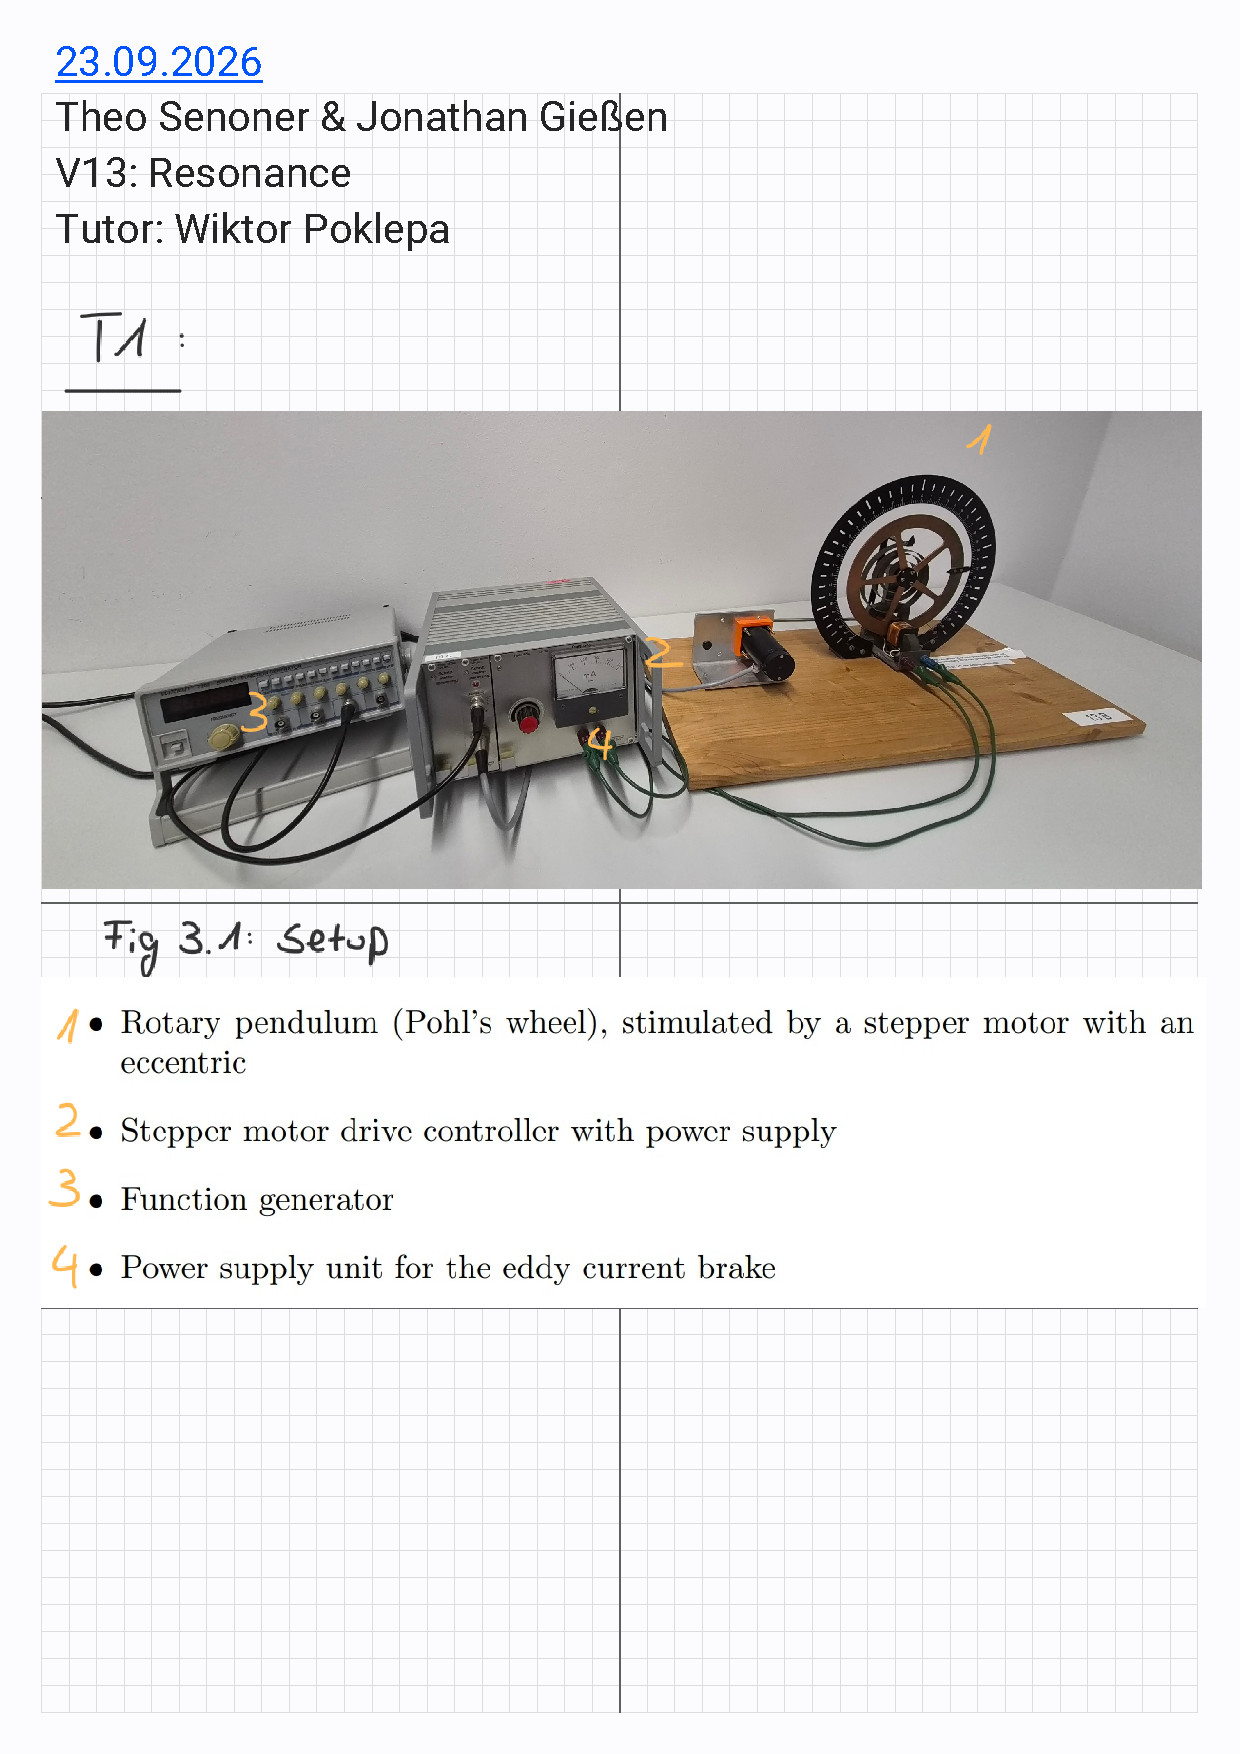
\includepdf[
    pages=-,
    width=\textwidth,
    height=0.95\textheight,
    keepaspectratio,
    pagecommand={\thispagestyle{scrheadings}},
    pagecommand*={\thispagestyle{scrheadings}}
]{../Messprotokoll 13.pdf}



\subsection{Procedure}
The measuring process is divided into four main tasks to analyze both free and forced oscillations:

\begin{enumerate}
    \item \textbf{Period of the Free Oscillator:} Determine the oscillation period $T_0$ of the undamped, free torsion pendulum by measuring the duration of 20 full oscillation periods. Repeat this measurement three times.
    \item \textbf{Transient Time and Damping:} Activate the eddy current brake. Find two specific damping currents: one where the amplitude decays to 5\% of its initial value after about 10 oscillations, and another where it decays to 5\% after about 15 oscillations. Measure the transient time for both settings.
    \item \textbf{Amplitude Decay:} For the two selected damping currents, release the pendulum from a reversal point at $t=0$ and record the amplitude after every full period to document the exponential decay.
    \item \textbf{Forced Oscillations:} Excite the pendulum with the stepper motor. Measure the stationary amplitude as a function of the excitation frequency (generator frequency from 300\,Hz to 4000\,Hz) for both damping settings. Wait for the transient process to finish before each reading, and use smaller frequency steps (50\,Hz) near the resonance peak to accurately determine the resonance frequency and the Full Width at Half Maximum (FWHM).
\end{enumerate}


\section{Examination of the Results}

\subsection{Excersise 1: Period of the Free Oscillator}

We measured the oscillation period of the undamped torsion pendulum by timing 20 full oscillations. The measurements were repeated three times to ensure accuracy. The results are summarized in Table \ref{tab:period_measurements}.
The measured Values are:
\begin{table}[H]
    \centering
    \caption{Measured oscillation periods for 20 full oscillations of the undamped torsion pendulum.}\label{tab:period_measurements}
    \begin{tabular}{lcc}
        \toprule
        \textbf{Measurement} & \textbf{Time for 20 Oscillations (s)} & \textbf{Calculated Period $T_0$ (s)} \\
        \midrule
        1 & \num{39.61(0.25)} & \num{1.981(13)} \\
        2 & \num{39.72(0.25)} & \num{1.986(13)} \\
        3 & \num{39.73(0.25)} & \num{1.987(13)} \\
        \bottomrule
    \end{tabular}
\end{table}


With the error calculation of:

\begin{equation}
    \Delta T_0 = \sqrt{\Delta T_\text{stat}^2 + \Delta T_\text{sys}^2} = \sqrt{(0.002)^2 + (0.013)^2} \approx 0.014\,\text{s}
\end{equation}

The Mean of the measured periods is:
\begin{equation}
    T_0 = \qty{1.984}{13}
\end{equation}

\begin{resultbox}[Result]
    The oscillation period of the undamped torsion pendulum is determined to be:
    \begin{align}
        T_0 = \qty{1.984(14)}{\second}\\
        f_0 = \qty{0.504(4)}{\hertz}
    \end{align}
\end{resultbox}

\bigskip
\subsection{Excersise 2: Evaluate the damping constant $\delta$}

The damping constant $\delta$ can be determined by measuring the amplitude with respect to the number os oscilations. For each damping current of the eddy current brake, the average of two measurements of the amplitude was determined after each full oscillation until it reached > 5\% of the initial amplitude. The results are plotted logarithmically to determine the damping constant $\delta$ from the slope of the fit. 

The error of the amplitude is estimated to be $\Delta a = 0.2\,\text{Skt}$, which corresponds to the uncertainty of the measurement due to the scale division of the torsion pendulum.

     
\begin{figure}[H]
    \centering
    \begin{subfigure}[b \ref{fig:amplitude_decay_280_appendix}]{0.48\textwidth}
        \centering
        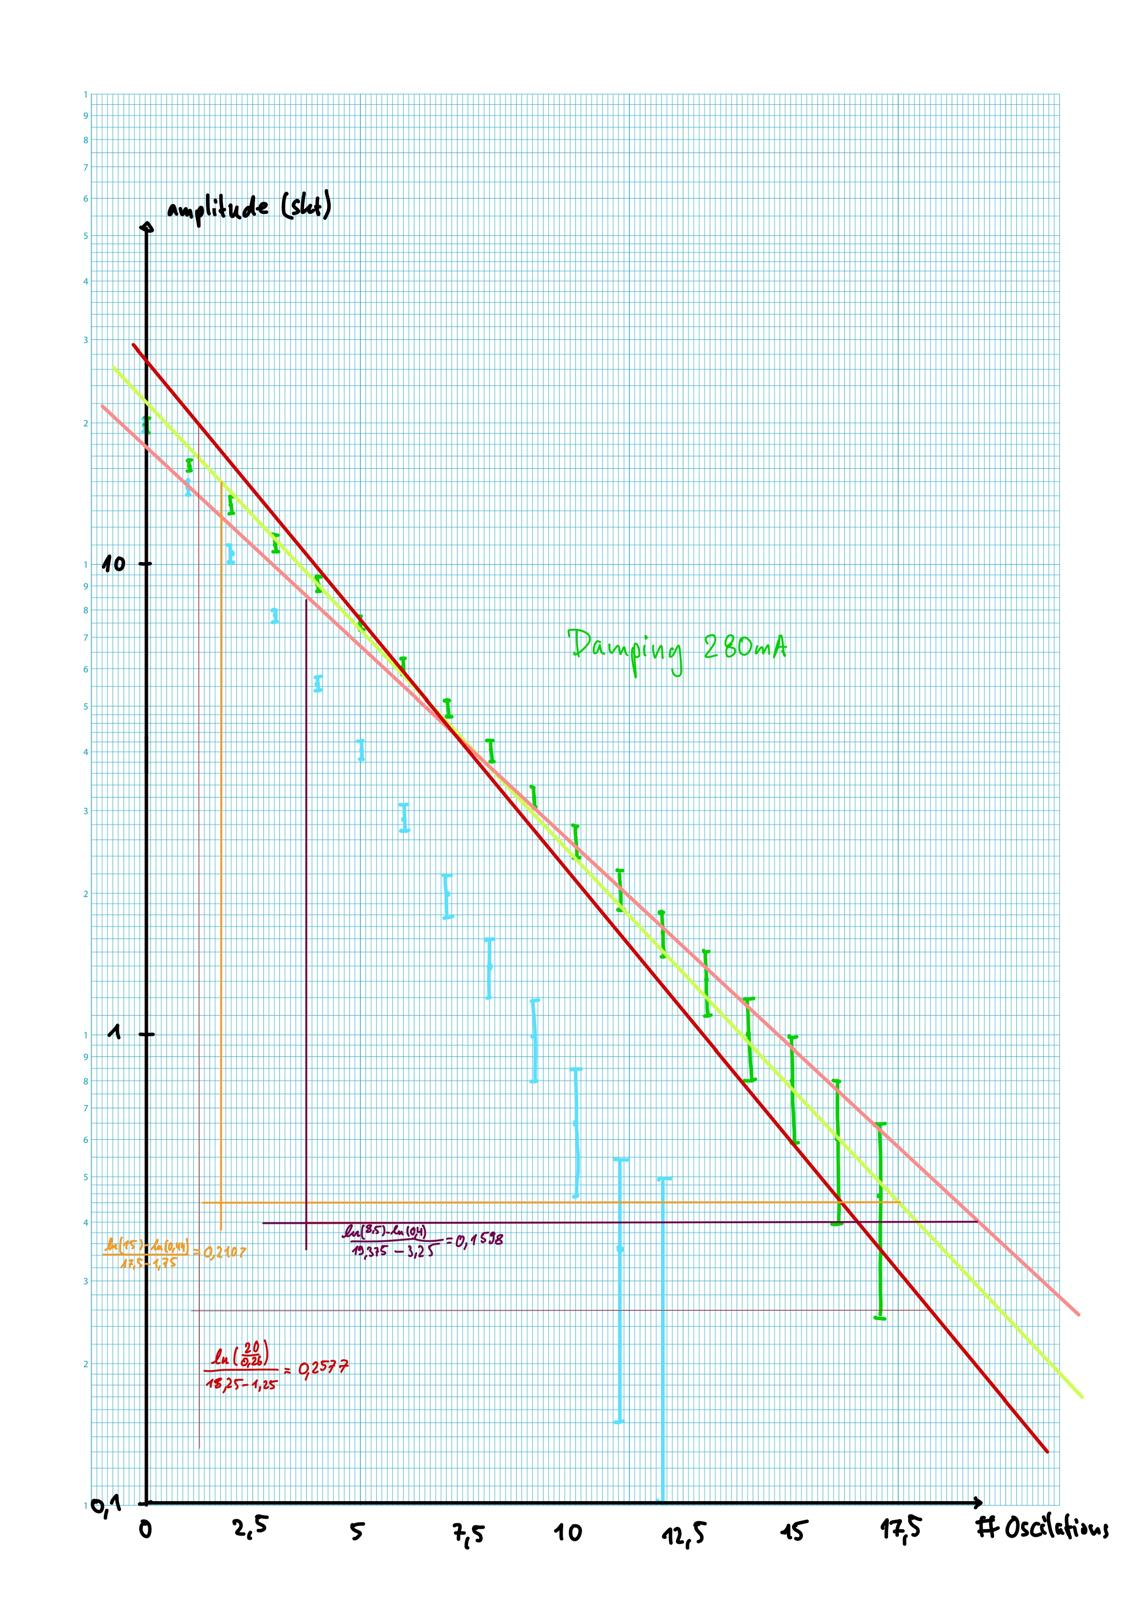
\includegraphics[width=\textwidth]{img/A2_280mA.jpeg}
        \caption{Damping current: 280\,mA.}\label{fig:amplitude_decay_280}
    \end{subfigure}
    \hfill
    \begin{subfigure}[b \ref{fig:amplitude_decay_360_appendix}]{0.48\textwidth}
        \centering
        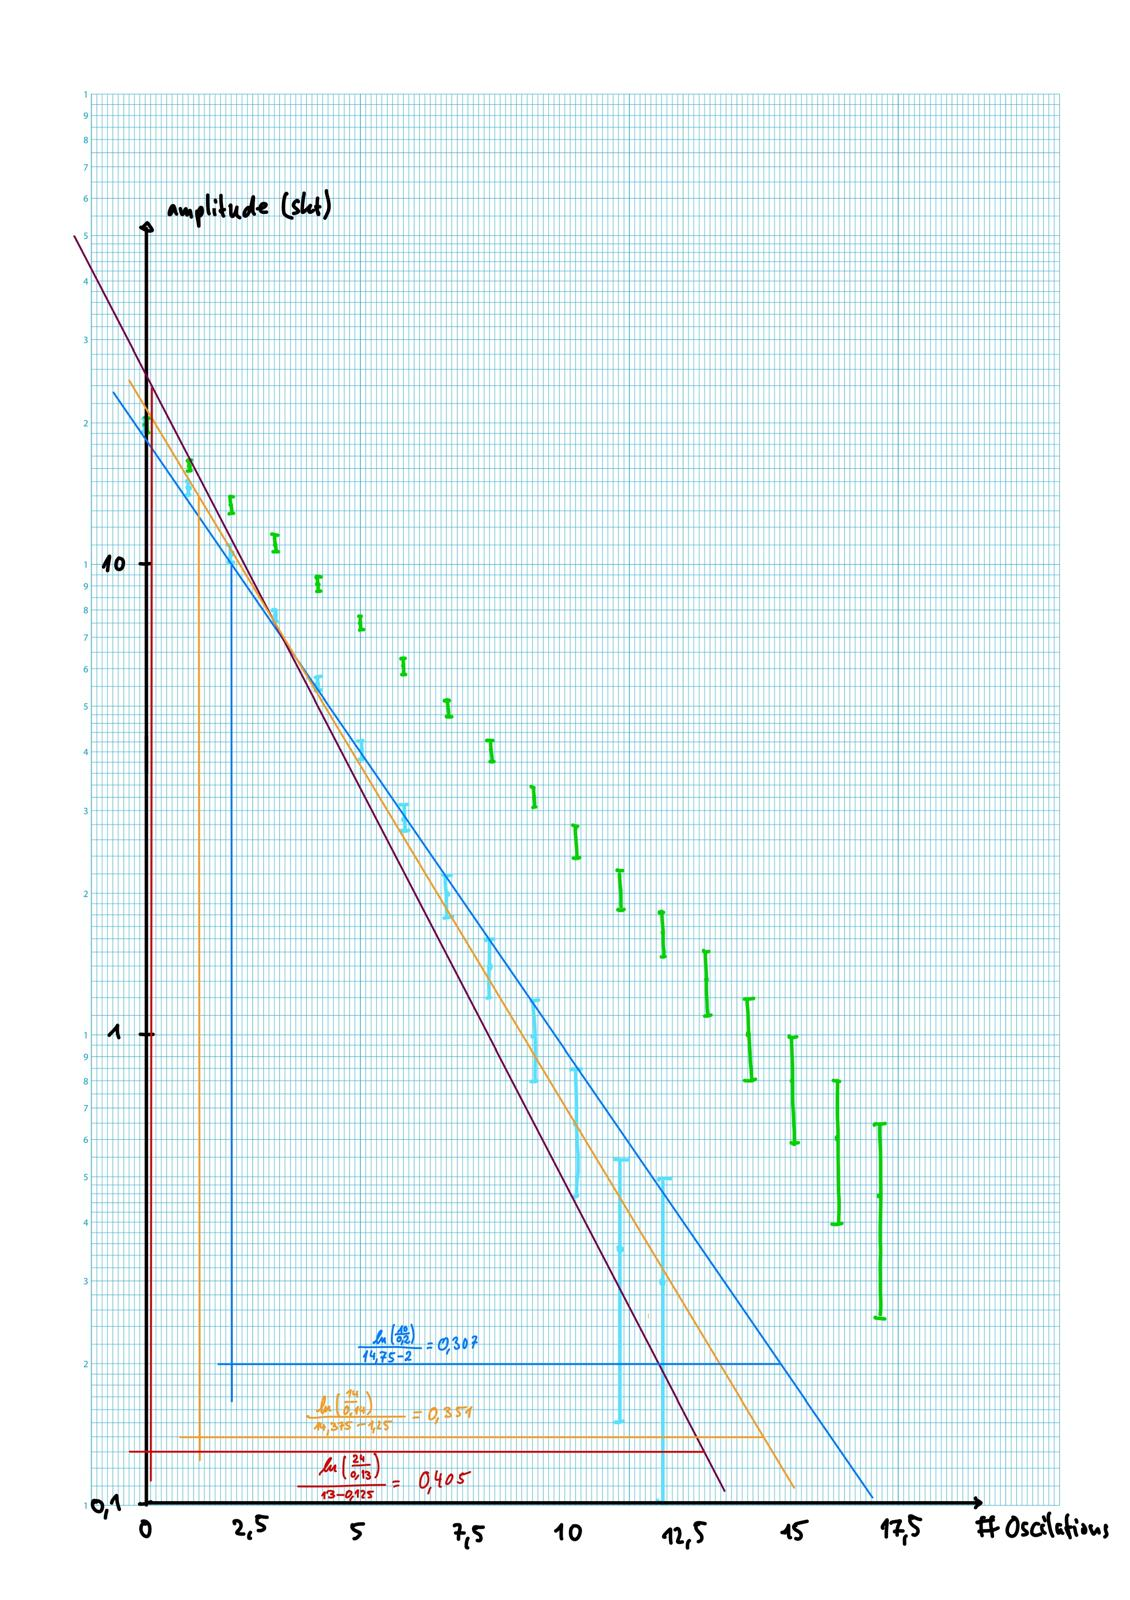
\includegraphics[width=\textwidth]{img/A2_360mA.jpeg}
        \caption{Damping current: 360\,mA.}\label{fig:amplitude_decay_360}
    \end{subfigure}
    \caption{Determination of the damping coefficient for two damping currents.}\label{fig:amplitude_decay}
\end{figure}

\footnotetext[1]{The plots are listed in full scale in the appendix}

from the slope of the linear fit, the damping constants are:
\begin{enumerate}
    \item for 280\,mA: $(\num{-0.21(5)})\,\frac{1}{\text{Oscilations}}$
    \item for 360\,mA: $(\num{-0.35(5)})\,\frac{1}{\text{Oscilations}}$
\end{enumerate}

Since the oscillation period $T_0$ is known, the damping constants can be converted to units of $\frac{1}{\text{s}}$:
\begin{align}
    \delta_{280} = \frac{-0.21(5)}{T_0} = \qty{-0.11(3)}{\per\second}\\
    \delta_{360} = \frac{-0.35(5)}{T_0} = \qty{-0.18(3)}{\per\second}
\end{align}

\begin{resultbox}[Result]
    The damping constants for the two damping currents are determined to be:
    \begin{align}
        \delta_{280} = \qty{-0.11(3)}{\per\second}\\
        \delta_{360} = \qty{-0.18(3)}{\per\second}
    \end{align}
\end{resultbox}

\subsection{Excersise 3: Forced Oscillation and Resonance}
The resonance curves are drawn for both damping currents. 

\begin{figure}[H]
    \centering
    \begin{subfigure}[b]{0.48\textwidth}
        \centering
        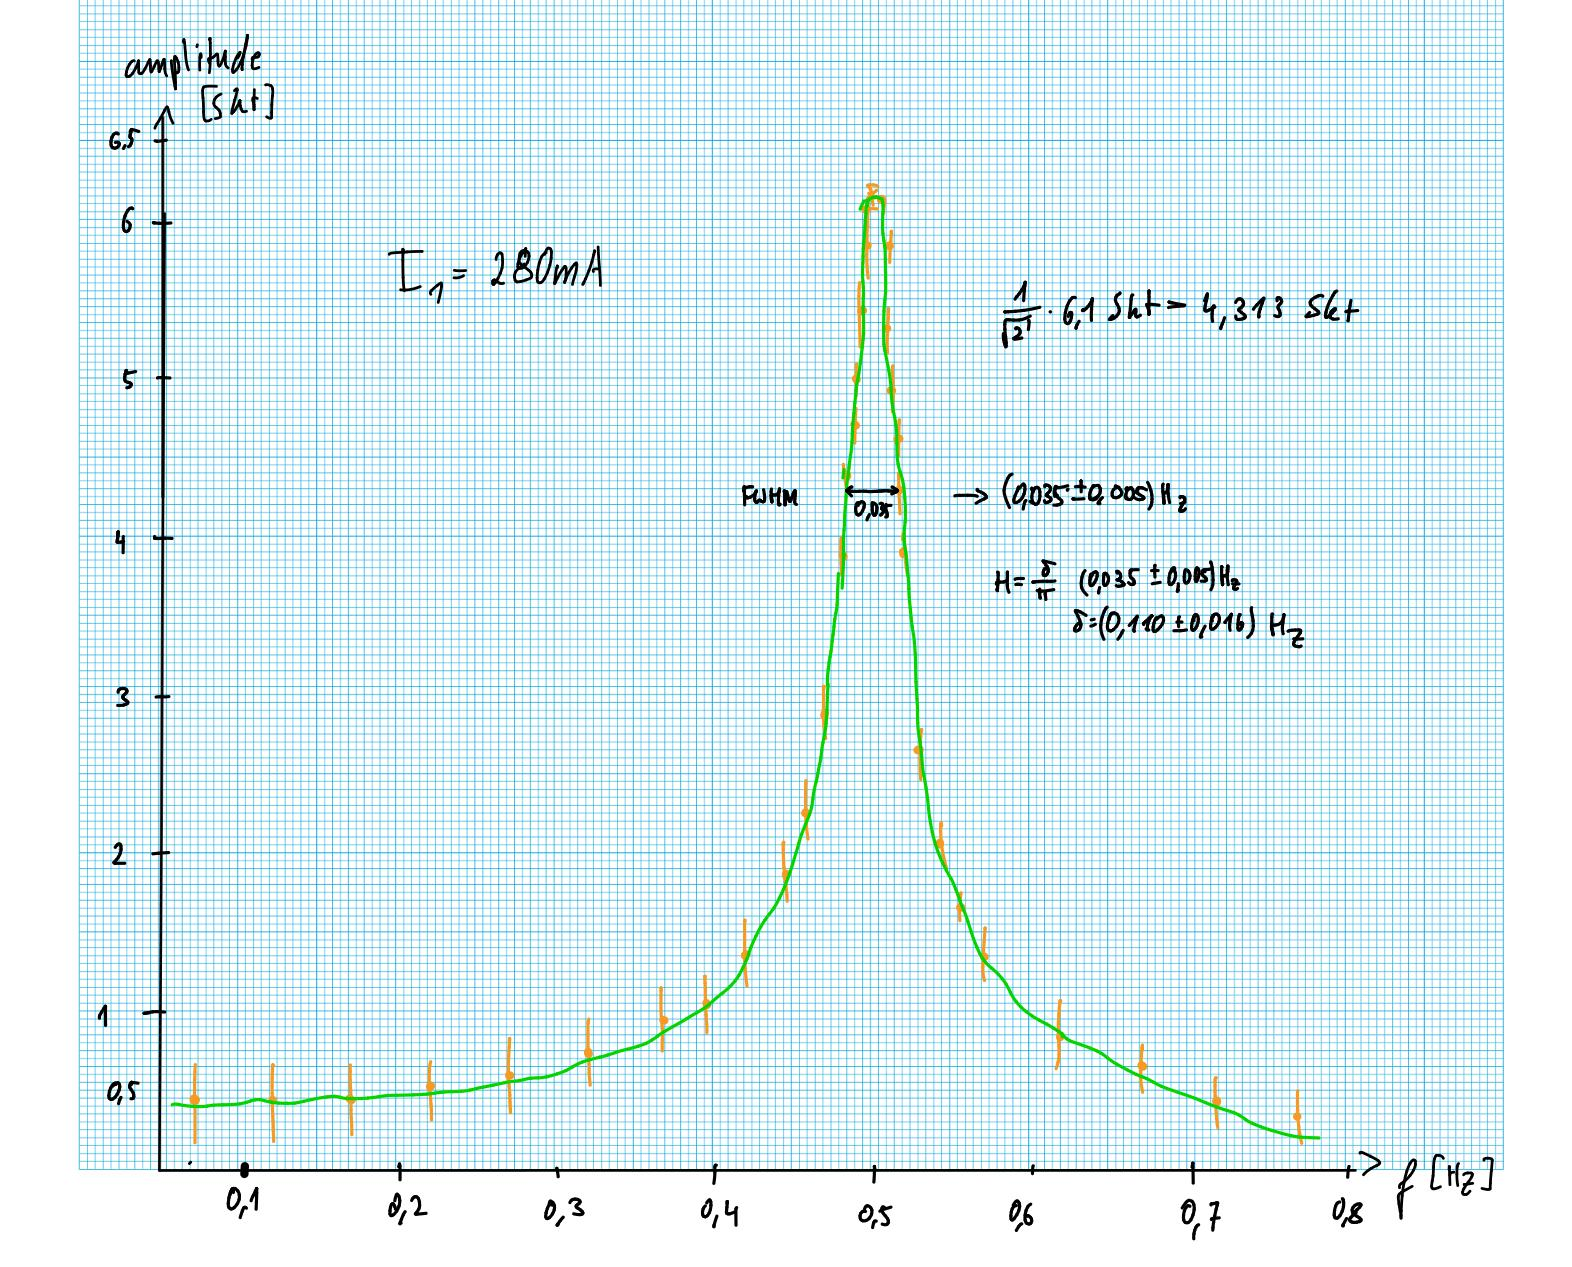
\includegraphics[width=\textwidth]{img/A3_280mA.jpeg}
        \caption{Damping current: 280\,mA.}\label{fig:resonance_curve_280}
    \end{subfigure}
    \hfill
    \begin{subfigure}[b]{0.48\textwidth}
        \centering
        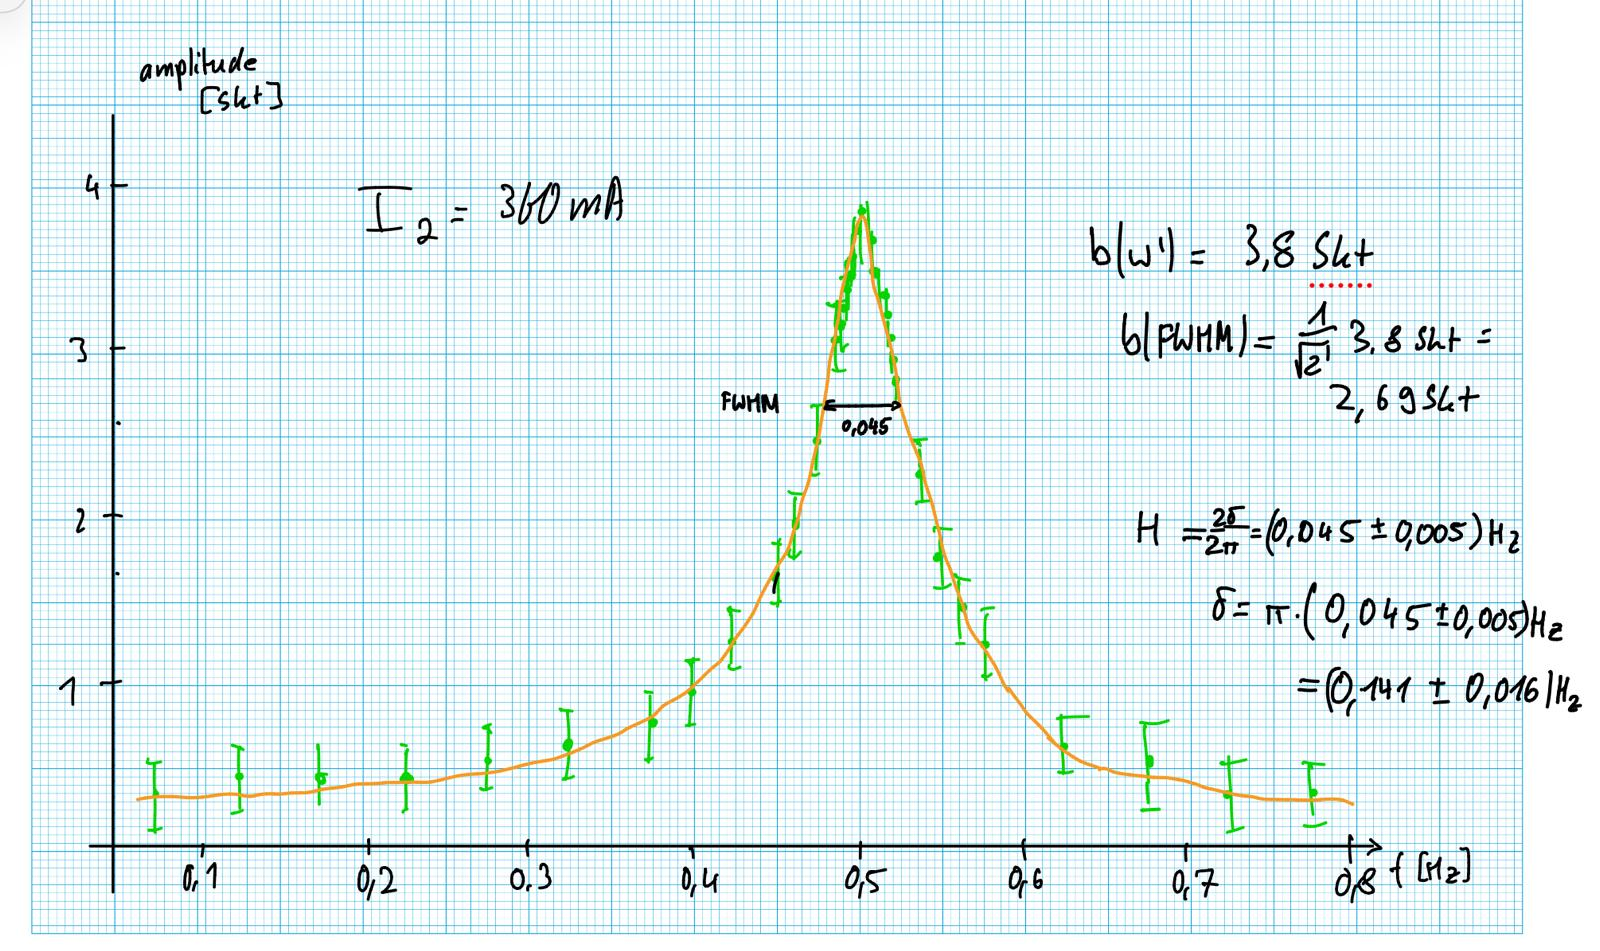
\includegraphics[width=\textwidth]{img/A3_360mA.jpeg}
        \caption{Damping current: 360\,mA.}\label{fig:resonance_curve_360}
    \end{subfigure}
    \caption{Resonance curves for two damping currents. The resonance frequency and the Full Width at Half Maximum (FWHM) are determined from the plots.}\label{fig:resonance_curves}
\end{figure}


The corrollation between the damping constant $\delta$ and the FWHM $H$ is given by equation~\ref{eq:FWHM}, the measured width has to be multiplied by $\pi$ to get the damping constant.


The measured values for the resonance frequency and the Full Width at Half Maximum (FWHM) are summarized in Table~\ref{tab:resonance_measurements}. 


\begin{table}[H]
    \centering
    \caption{Measured resonance frequencies and Full Width at Half Maximum (FWHM) for two damping currents.}\label{tab:resonance_measurements}
    \begin{tabular}{lcc}
        \toprule
        \textbf{Damping Current} & \textbf{Resonance Frequency $f$ (Hz)} & \textbf{$\delta$ (Hz)} \\
        \midrule
        280\,mA & \num{0.505(5)} & \num{0.110(16)} \\
        360\,mA & \num{0.506(5)} & \num{0.141(16)} \\
        \bottomrule
    \end{tabular}
\end{table}

The natural frequency $f_0 = \qty{0.504(4)}{\hertz}$ is slightly lower than the measured resonance frequencies, which is consistent with the theoretical expectation that the resonance frequency is slightly lower than the natural frequency due to damping.

The resonance step-up (quality factor) (Equation~\ref{eq:Quality-factor}) tells how much the amplitude is amplified at resonance compared to the static amplitude.

The quality factor can also be calculated using the measured values of the resonance frequency and the damping constant. 

\begin{align}
    Q_{damping} = \frac{\omega_0}{2\delta}\\
    Q_{measured} = \frac{b(\omega')}{b(\omega \rightarrow 0)}
\end{align}

\begin{table}[H]
    \centering
    \caption{Quality factor for two damping currents.}\label{tab:quality_factor}
    \begin{tabular}{lcc}
        \toprule
        \textbf{Damping Current} & \textbf{$Q_{damping}$} & \textbf{$Q_{measured}$} \\
        \midrule
        280\,mA & \num{15(4)} & \num{15(8)}\\
        360\,mA & \num{9.0(13)} & \num{9(5)}\\
        \bottomrule
    \end{tabular}
\end{table}

The difference between the theoretical and measured damping constants is:

\begin{equation}
    \sigma \delta = \frac{\delta_{measured} - \delta_{damping}}{\sqrt{\Delta \delta_{damping} ^2 + \Delta \delta_{measured}^2}} = \begin{cases}
        \sigma \delta_{280} \approx 0.14\\
        \sigma \delta_{360} \approx 1.18
    \end{cases}
\end{equation}

\begin{resultbox}[Result]
    The measured resonance frequencies and Full Width at Half Maximum (FWHM) for the two damping currents are:
    \begin{align}
        f_{280} = \qty{0.505(5)}{\hertz}\\
        f_{360} = \qty{0.506(5)}{\hertz}\\
        \delta_{280} = \qty{0.110(16)}{\hertz} \Rightarrow 0.14\sigma\\
        \delta_{360} = \qty{0.141(16)}{\hertz} \Rightarrow 1.18\sigma
    \end{align} 

    The quality factors for the two damping currents are:
    \begin{align}
        Q_{280} = \num{15(4)}\\
        Q_{360} = \num{9.0(13)}
    \end{align}
\end{resultbox}

\section{Conclusion}
In this experiment, we investigated the fundamental dynamic properties of a torsion pendulum, focusing on both free, damped oscillations and forced oscillations under periodic external torque. We determined the oscillation period of the undamped torsion pendulum, measured the damping constants for two different damping currents, and analyzed the resonance behavior during forced oscillations. The measured resonance frequencies and Full Width at Half Maximum (FWHM) were consistent with theoretical expectations, and the quality factors for the two damping currents were determined. With a sigma-deviation of 0.14 and 1.18. The bigger deviation can be explained by the approximation using the Lorentz profile, which is only exact in the limit of small damping. The damping with $I_2 = 360\,\text{mA}$ shows a larger deviation than the damping with $I_1 = 280\,\text{mA}$.
Using python, i've fitted the data to the exact Breit-Wigner function, which is the exact solution of the forced oscillation.
\begin{equation}
    A(\omega) = \frac{A_0 \cdot \omega_0^2}{\sqrt{{\left(\omega_0^2 - \omega^2 \right)}^2 + {\left( 2\gamma\omega \right)}^2}}
\end{equation}

using this fit, the damping constant is given by $\gamma$ and the resonance frequency is given by $\omega_0$. The results are:
\begin{align}
    \gamma_{280} = \qty{0.0981}{\hertz} \\
    \gamma_{360} = \qty{0.165}{\hertz} 
\end{align}

\begin{figure}[H]
    \centering
    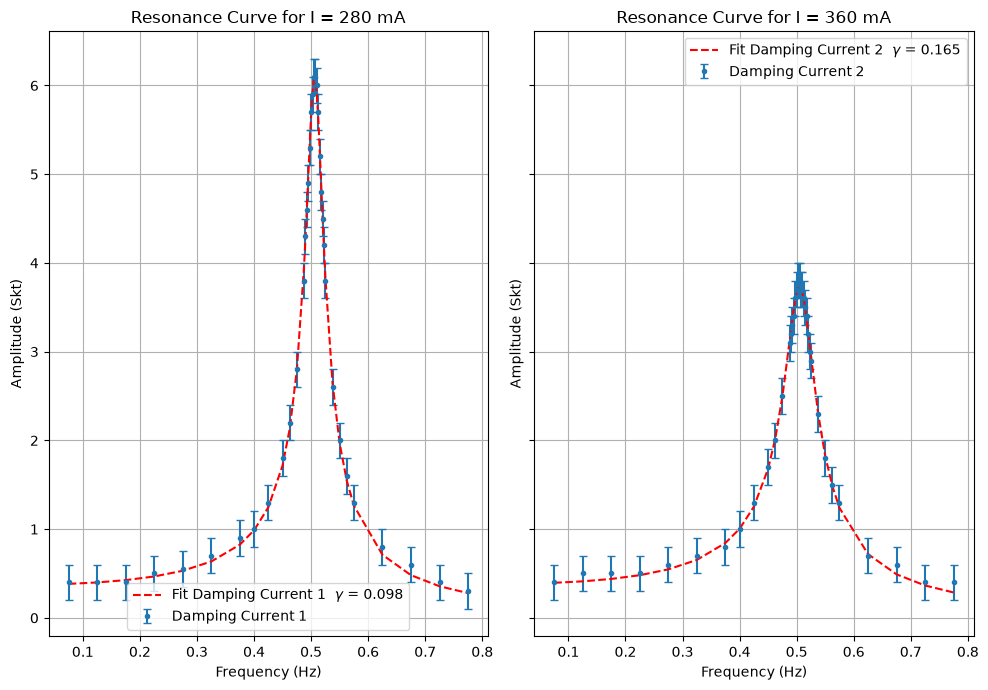
\includegraphics[width=0.95\textwidth]{img/A3_pyhton.png}
    \caption{Resonance curve for a damping current of 280\,mA and 360\,mA fitted with the exact Breit-Wigner function.}\label{fig:resonance_curve_fit}
\end{figure}

This sows the exact deviation by assuming a lorentz profile.

Overall, the experiment provided valuable insights into the behavior of oscillating systems and their response to external forces.



\clearpage

\listoffigures


\listoftables

\begin{thebibliography}{5}
    \bibitem{PAPskript} Dr. J.Wagner, \emph{Physikalisches Anfängerpraktikum}, Stand 11/2024
    \bibitem{ilberg1988physikalisches} W. Ilberg, M. Krötzsch, \emph{Physikalisches Praktikum für Anfänger}, BSB B. G. Teubner Verlagsgesellschaft, Leipzig (1985).
\end{thebibliography}



\appendix
\section{Plots}

\begin{figure}[H]
    \centering
    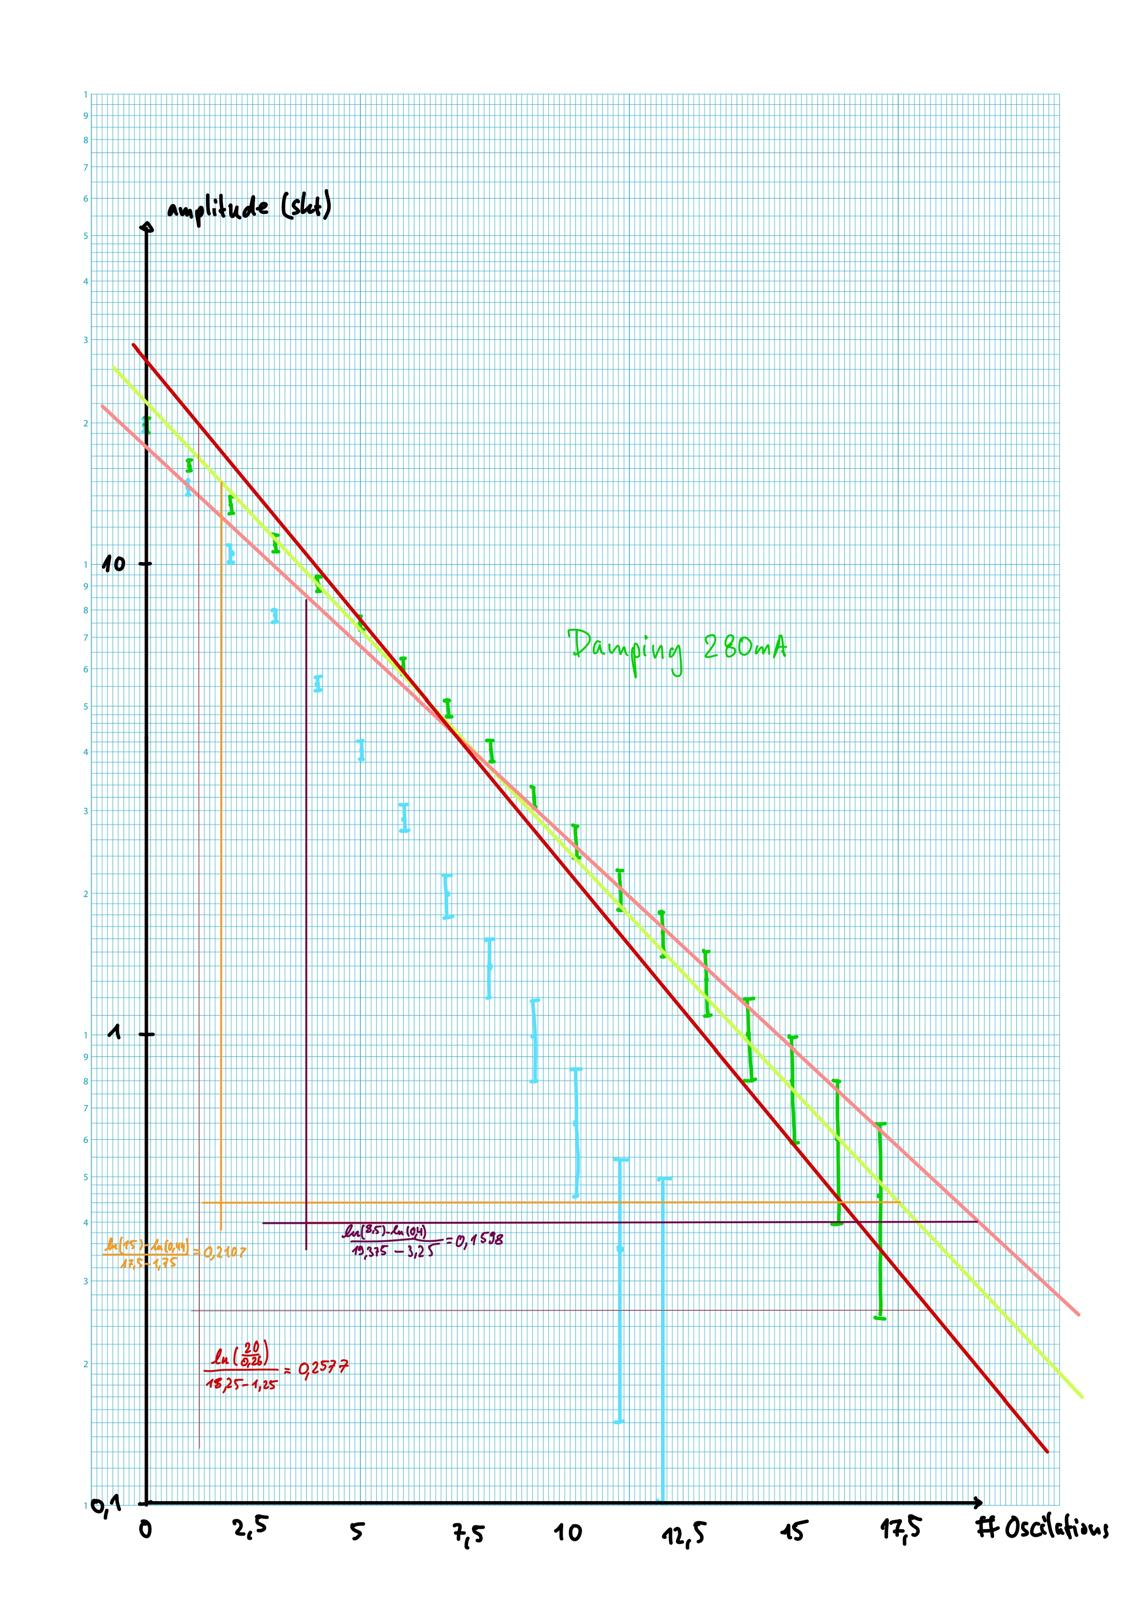
\includegraphics[width=\textwidth]{img/A2_280mA.jpeg}
    \caption{Amplitude decay for a damping current of 280\,mA.}\label{fig:amplitude_decay_280_appendix}
\end{figure}

\begin{figure}[H]
    \centering
    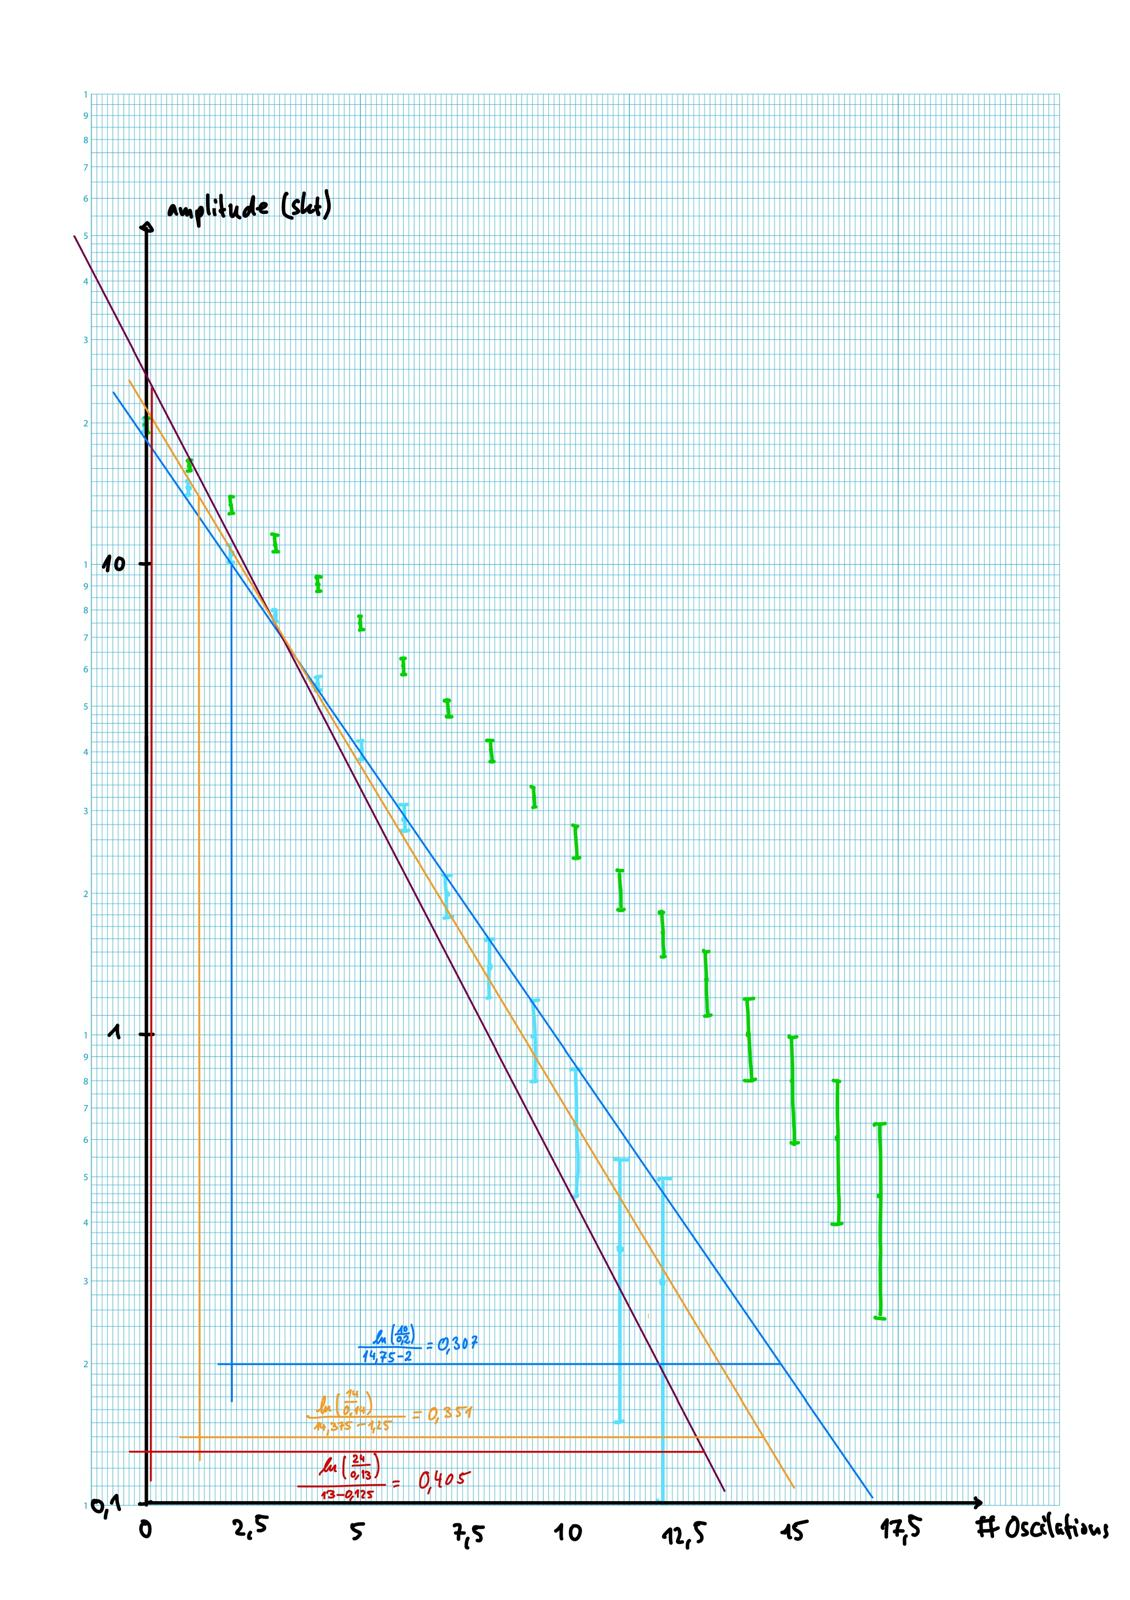
\includegraphics[width=\textwidth]{img/A2_360mA.jpeg}
    \caption{Amplitude decay for a damping current of 360\,mA.}\label{fig:amplitude_decay_360_appendix}
\end{figure}

\begin{figure}[H]
    \centering
    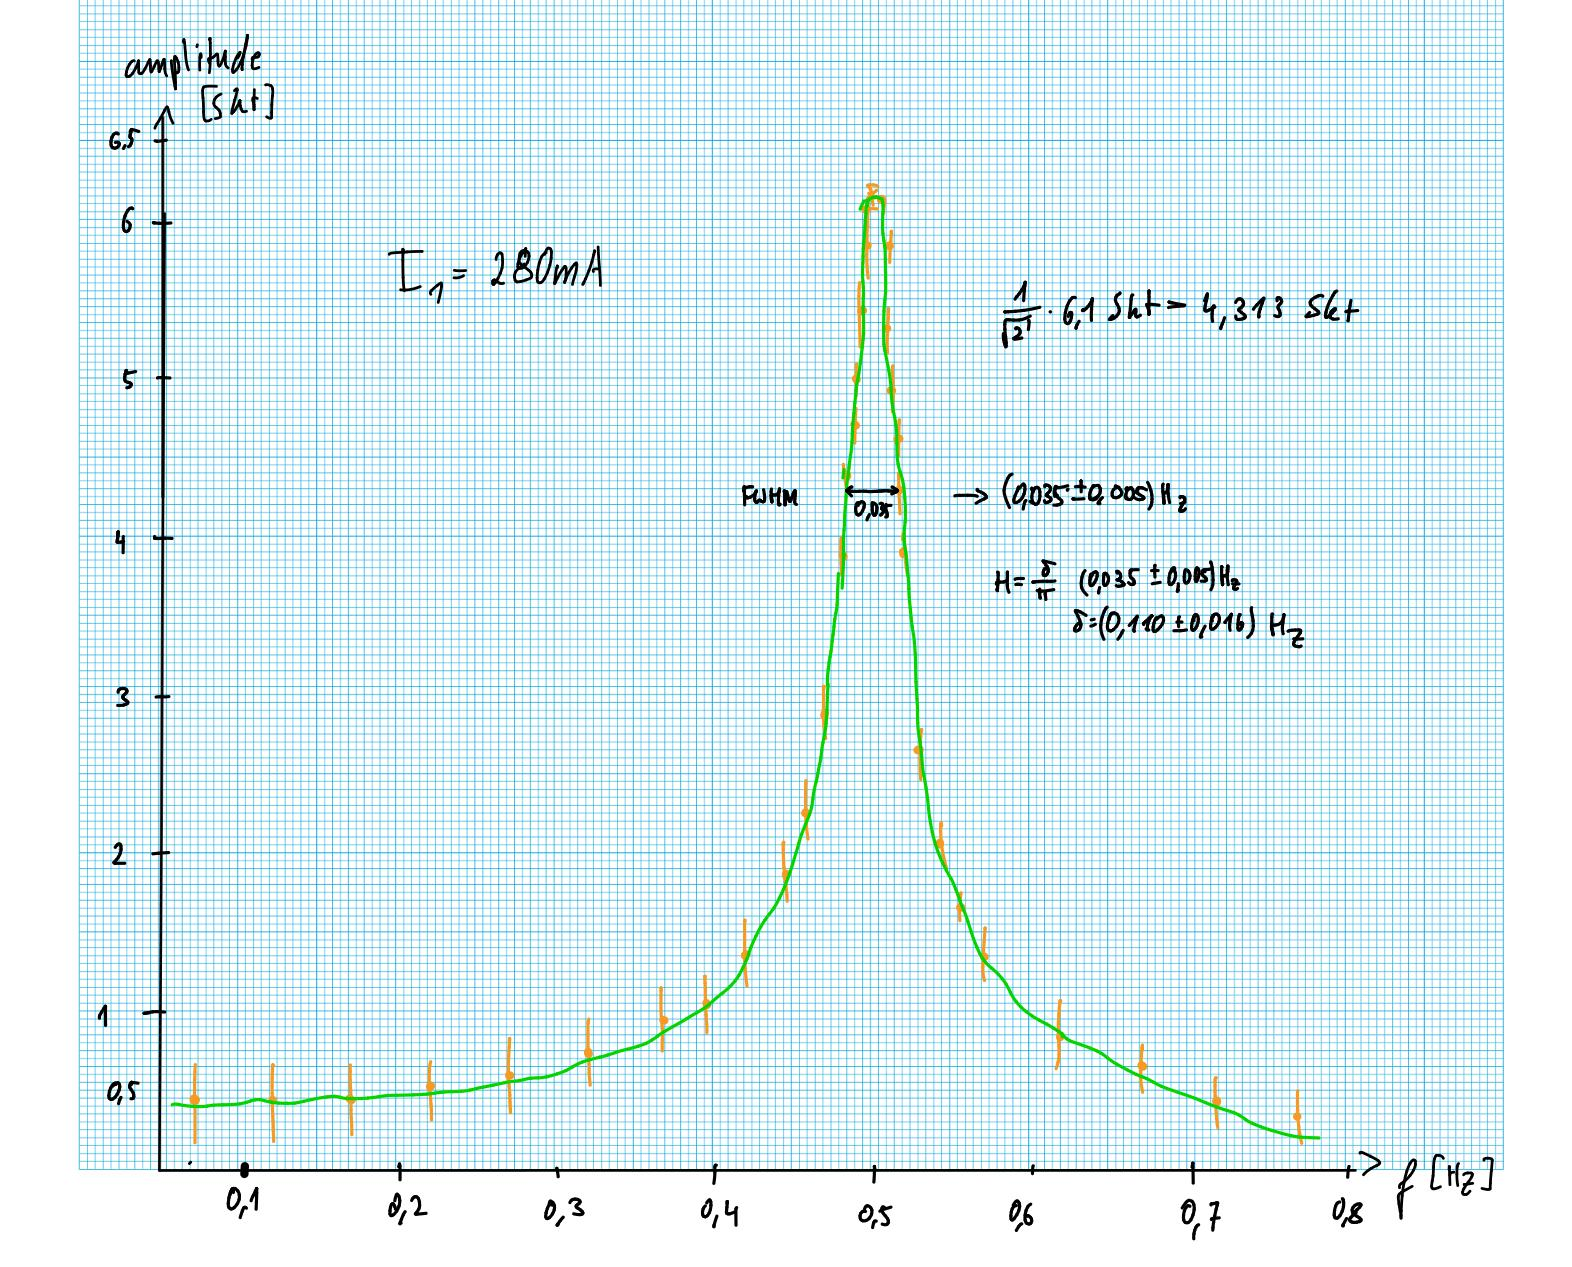
\includegraphics[width=\textwidth]{img/A3_280mA.jpeg}
    \caption{Resonance curve for a damping current of 280\,mA.}\label{fig:resonance_curve_280_appendix}
\end{figure}

\begin{figure}[H]
    \centering
    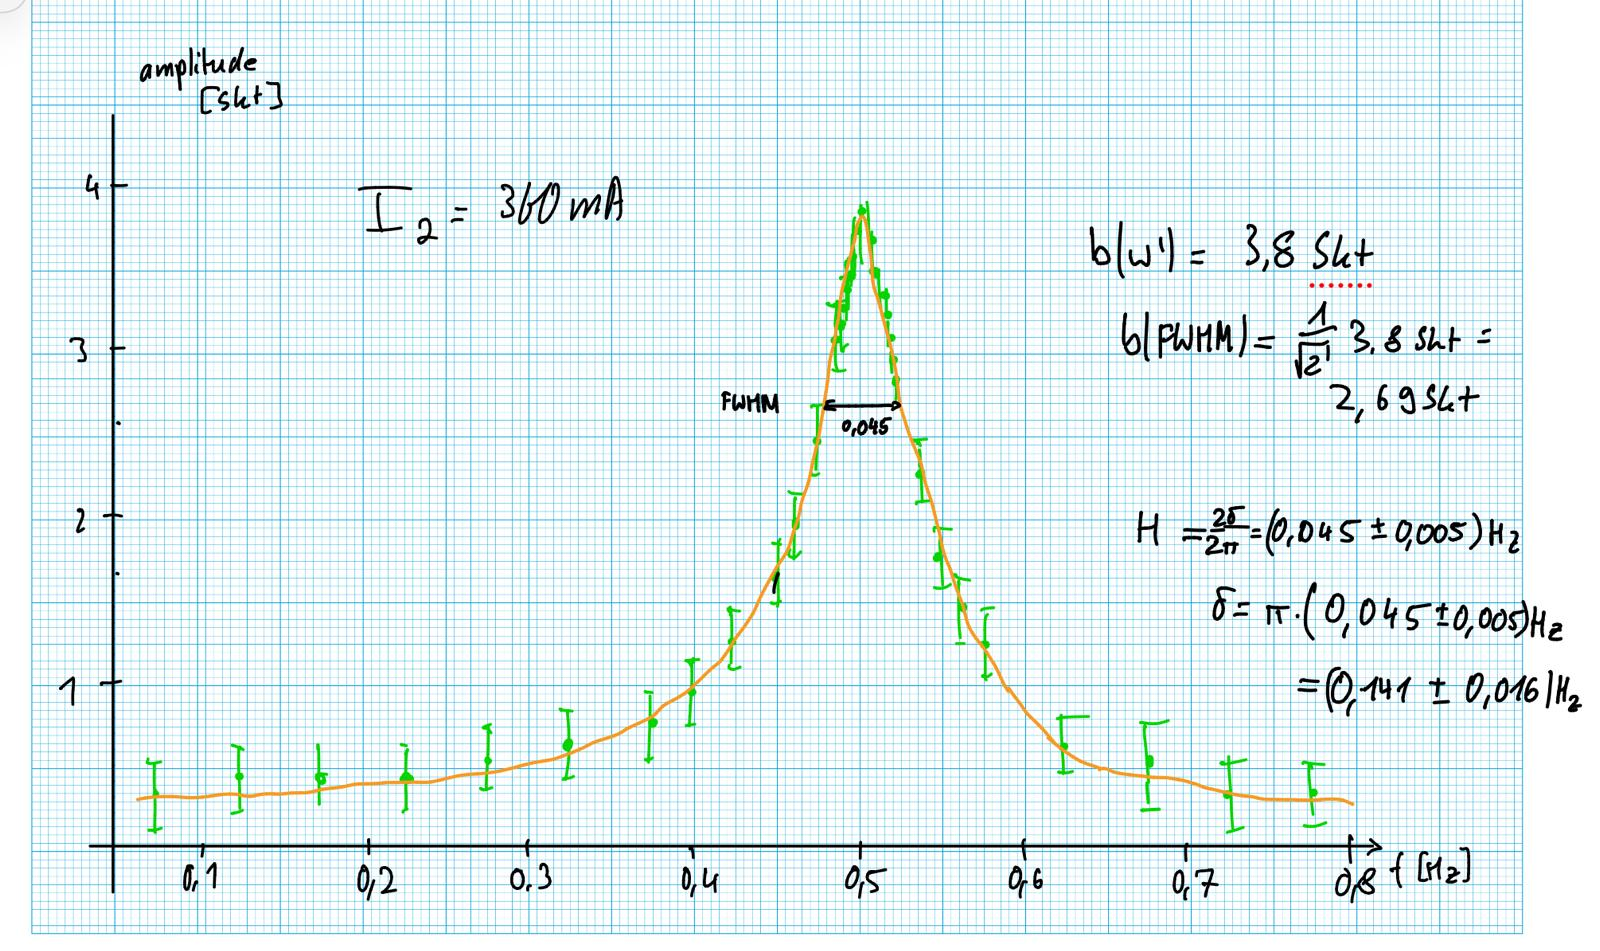
\includegraphics[width=\textwidth]{img/A3_360mA.jpeg}
    \caption{Resonance curve for a damping current of 360\,mA.}\label{fig:resonance_curve_360_appendix}
\end{figure}


\section{Python Code}
The following code was used to analyze the data and generate the plots in this report. It includes the necessary functions for fitting the data to the theoretical models and calculating the relevant parameters.



    
    \(T_0\) berechnen

    \begin{tcolorbox}[breakable, size=fbox, boxrule=1pt, pad at break*=1mm,colback=cellbackground, colframe=cellborder]
\prompt{In}{incolor}{1}{\boxspacing}
\begin{Verbatim}[commandchars=\\\{\}]
\PY{k+kn}{import}\PY{+w}{ }\PY{n+nn}{numpy}\PY{+w}{ }\PY{k}{as}\PY{+w}{ }\PY{n+nn}{np}
\PY{k+kn}{import}\PY{+w}{ }\PY{n+nn}{uncertainties}\PY{+w}{ }\PY{k}{as}\PY{+w}{ }\PY{n+nn}{unc}
\PY{k+kn}{import}\PY{+w}{ }\PY{n+nn}{uncertainties}\PY{n+nn}{.}\PY{n+nn}{unumpy}\PY{+w}{ }\PY{k}{as}\PY{+w}{ }\PY{n+nn}{unp}
\PY{k+kn}{import}\PY{+w}{ }\PY{n+nn}{matplotlib}\PY{n+nn}{.}\PY{n+nn}{pyplot}\PY{+w}{ }\PY{k}{as}\PY{+w}{ }\PY{n+nn}{plt}
\PY{k+kn}{from}\PY{+w}{ }\PY{n+nn}{scipy}\PY{n+nn}{.}\PY{n+nn}{optimize}\PY{+w}{ }\PY{k+kn}{import} \PY{n}{curve\PYZus{}fit}
\end{Verbatim}
\end{tcolorbox}

    \begin{tcolorbox}[breakable, size=fbox, boxrule=1pt, pad at break*=1mm,colback=cellbackground, colframe=cellborder]
\prompt{In}{incolor}{2}{\boxspacing}
\begin{Verbatim}[commandchars=\\\{\}]
\PY{n}{T} \PY{o}{=} \PY{n}{np}\PY{o}{.}\PY{n}{array}\PY{p}{(}\PY{p}{[}\PY{l+m+mf}{39.61}\PY{p}{,} \PY{l+m+mf}{39.72}\PY{p}{,} \PY{l+m+mf}{39.73}\PY{p}{]}\PY{p}{)}

\PY{n}{unc\PYZus{}T} \PY{o}{=} \PY{l+m+mf}{0.25}

\PY{n}{T} \PY{o}{=} \PY{n}{unp}\PY{o}{.}\PY{n}{uarray}\PY{p}{(}\PY{n}{T}\PY{p}{,} \PY{n}{unc\PYZus{}T}\PY{p}{)}
\PY{n}{T\PYZus{}0} \PY{o}{=} \PY{n}{T}\PY{o}{/}\PY{l+m+mi}{20}
\PY{n}{T\PYZus{}0}
\PY{n}{T\PYZus{}fin\PYZus{}err} \PY{o}{=} \PY{n}{np}\PY{o}{.}\PY{n}{sqrt}\PY{p}{(}\PY{p}{(}\PY{n}{np}\PY{o}{.}\PY{n}{std}\PY{p}{(}\PY{n}{unp}\PY{o}{.}\PY{n}{nominal\PYZus{}values}\PY{p}{(}\PY{n}{T\PYZus{}0}\PY{p}{)}\PY{p}{,} \PY{n}{ddof}\PY{o}{=}\PY{l+m+mi}{1}\PY{p}{)} \PY{o}{/} \PY{n}{np}\PY{o}{.}\PY{n}{sqrt}\PY{p}{(}\PY{n+nb}{len}\PY{p}{(}\PY{n}{T\PYZus{}0}\PY{p}{)}\PY{p}{)}\PY{p}{)}\PY{o}{*}\PY{o}{*}\PY{l+m+mi}{2} \PY{o}{+} \PY{l+m+mf}{0.013}\PY{o}{*}\PY{o}{*}\PY{l+m+mi}{2}\PY{p}{)}
\PY{n}{T\PYZus{}fin} \PY{o}{=} \PY{n}{unc}\PY{o}{.}\PY{n}{ufloat}\PY{p}{(}
    \PY{n+nb}{float}\PY{p}{(}\PY{n}{np}\PY{o}{.}\PY{n}{mean}\PY{p}{(}\PY{n}{unp}\PY{o}{.}\PY{n}{nominal\PYZus{}values}\PY{p}{(}\PY{n}{T\PYZus{}0}\PY{p}{)}\PY{p}{)}\PY{p}{)}\PY{p}{,}
    \PY{n+nb}{float}\PY{p}{(}\PY{n}{T\PYZus{}fin\PYZus{}err}\PY{p}{)}
\PY{p}{)}
\PY{n+nb}{print}\PY{p}{(}\PY{n}{T\PYZus{}fin}\PY{p}{)}
\PY{n+nb}{print}\PY{p}{(}\PY{l+m+mi}{1}\PY{o}{/}\PY{n}{T\PYZus{}fin}\PY{p}{)}
\end{Verbatim}
\end{tcolorbox}

    \begin{Verbatim}[commandchars=\\\{\}]
1.984+/-0.013
0.5039+/-0.0033
    \end{Verbatim}

    \begin{tcolorbox}[breakable, size=fbox, boxrule=1pt, pad at break*=1mm,colback=cellbackground, colframe=cellborder]
\prompt{In}{incolor}{3}{\boxspacing}
\begin{Verbatim}[commandchars=\\\{\}]
\PY{n}{i1\PYZus{}run1} \PY{o}{=} \PY{p}{[}\PY{l+m+mf}{20.0}\PY{p}{,} \PY{l+m+mf}{16.5}\PY{p}{,} \PY{l+m+mf}{13.6}\PY{p}{,} \PY{l+m+mf}{11.2}\PY{p}{,} \PY{l+m+mf}{9.2}\PY{p}{,} \PY{l+m+mf}{7.6}\PY{p}{,} \PY{l+m+mf}{6.2}\PY{p}{,} \PY{l+m+mf}{5.0}\PY{p}{,} \PY{l+m+mf}{4.0}\PY{p}{,} \PY{l+m+mf}{3.2}\PY{p}{,} \PY{l+m+mf}{2.6}\PY{p}{,} \PY{l+m+mf}{2.1}\PY{p}{,} \PY{l+m+mf}{1.7}\PY{p}{,} \PY{l+m+mf}{1.3}\PY{p}{,} \PY{l+m+mf}{1.0}\PY{p}{,} \PY{l+m+mf}{0.8}\PY{p}{,} \PY{l+m+mf}{0.6}\PY{p}{,} \PY{l+m+mf}{0.5}\PY{p}{]}
\PY{n}{i1\PYZus{}run2} \PY{o}{=} \PY{p}{[}\PY{l+m+mf}{20.0}\PY{p}{,} \PY{l+m+mf}{16.2}\PY{p}{,} \PY{l+m+mf}{13.5}\PY{p}{,} \PY{l+m+mf}{11.1}\PY{p}{,} \PY{l+m+mf}{9.0}\PY{p}{,} \PY{l+m+mf}{7.4}\PY{p}{,} \PY{l+m+mf}{6.0}\PY{p}{,} \PY{l+m+mf}{5.0}\PY{p}{,} \PY{l+m+mf}{4.0}\PY{p}{,} \PY{l+m+mf}{3.2}\PY{p}{,} \PY{l+m+mf}{2.6}\PY{p}{,} \PY{l+m+mf}{2.0}\PY{p}{,} \PY{l+m+mf}{1.6}\PY{p}{,} \PY{l+m+mf}{1.3}\PY{p}{,} \PY{l+m+mf}{1.0}\PY{p}{,} \PY{l+m+mf}{0.8}\PY{p}{,} \PY{l+m+mf}{0.6}\PY{p}{,} \PY{l+m+mf}{0.4}\PY{p}{]}

\PY{n}{i2\PYZus{}run1} \PY{o}{=} \PY{p}{[}\PY{l+m+mf}{20.0}\PY{p}{,} \PY{l+m+mf}{14.6}\PY{p}{,} \PY{l+m+mf}{10.7}\PY{p}{,} \PY{l+m+mf}{7.8}\PY{p}{,} \PY{l+m+mf}{5.6}\PY{p}{,} \PY{l+m+mf}{4.1}\PY{p}{,} \PY{l+m+mf}{2.9}\PY{p}{,} \PY{l+m+mf}{2.0}\PY{p}{,} \PY{l+m+mf}{1.4}\PY{p}{,} \PY{l+m+mf}{1.0}\PY{p}{,} \PY{l+m+mf}{0.7}\PY{p}{,} \PY{l+m+mf}{0.5}\PY{p}{,} \PY{l+m+mf}{0.3}\PY{p}{]}
\PY{n}{i2\PYZus{}run2} \PY{o}{=} \PY{p}{[}\PY{l+m+mf}{20.0}\PY{p}{,} \PY{l+m+mf}{14.8}\PY{p}{,} \PY{l+m+mf}{10.7}\PY{p}{,} \PY{l+m+mf}{7.8}\PY{p}{,} \PY{l+m+mf}{5.6}\PY{p}{,} \PY{l+m+mf}{4.1}\PY{p}{,} \PY{l+m+mf}{2.9}\PY{p}{,} \PY{l+m+mf}{2.0}\PY{p}{,} \PY{l+m+mf}{1.4}\PY{p}{,} \PY{l+m+mf}{1.0}\PY{p}{,} \PY{l+m+mf}{0.6}\PY{p}{,} \PY{l+m+mf}{0.2}\PY{p}{]}

\PY{k}{def}\PY{+w}{ }\PY{n+nf}{calculate\PYZus{}averages}\PY{p}{(}\PY{n}{run1}\PY{p}{,} \PY{n}{run2}\PY{p}{,} \PY{n}{n\PYZus{}max}\PY{p}{)}\PY{p}{:}
    \PY{n}{averages} \PY{o}{=} \PY{p}{[}\PY{p}{]}
    \PY{k}{for} \PY{n}{i} \PY{o+ow}{in} \PY{n+nb}{range}\PY{p}{(}\PY{n}{n\PYZus{}max}\PY{p}{)}\PY{p}{:}
        \PY{n}{values} \PY{o}{=} \PY{p}{[}\PY{p}{]}
        \PY{k}{if} \PY{n}{i} \PY{o}{\PYZlt{}} \PY{n+nb}{len}\PY{p}{(}\PY{n}{run1}\PY{p}{)}\PY{p}{:} \PY{n}{values}\PY{o}{.}\PY{n}{append}\PY{p}{(}\PY{n}{run1}\PY{p}{[}\PY{n}{i}\PY{p}{]}\PY{p}{)}
        \PY{k}{if} \PY{n}{i} \PY{o}{\PYZlt{}} \PY{n+nb}{len}\PY{p}{(}\PY{n}{run2}\PY{p}{)}\PY{p}{:} \PY{n}{values}\PY{o}{.}\PY{n}{append}\PY{p}{(}\PY{n}{run2}\PY{p}{[}\PY{n}{i}\PY{p}{]}\PY{p}{)}
        
        \PY{k}{if} \PY{n}{values}\PY{p}{:}
            \PY{n}{avg} \PY{o}{=} \PY{n+nb}{sum}\PY{p}{(}\PY{n}{values}\PY{p}{)} \PY{o}{/} \PY{n+nb}{len}\PY{p}{(}\PY{n}{values}\PY{p}{)}
            \PY{n}{averages}\PY{o}{.}\PY{n}{append}\PY{p}{(}\PY{n}{avg}\PY{p}{)}
        \PY{k}{else}\PY{p}{:}
            \PY{n}{averages}\PY{o}{.}\PY{n}{append}\PY{p}{(}\PY{k+kc}{None}\PY{p}{)}
    \PY{k}{return} \PY{n}{averages}



\PY{c+c1}{\PYZsh{} Process averages}
\PY{n}{i1\PYZus{}avg} \PY{o}{=} \PY{n}{calculate\PYZus{}averages}\PY{p}{(}\PY{n}{i1\PYZus{}run1}\PY{p}{,} \PY{n}{i1\PYZus{}run2}\PY{p}{,} \PY{n+nb}{len}\PY{p}{(}\PY{n}{i1\PYZus{}run1}\PY{p}{)}\PY{p}{)}
\PY{n}{i2\PYZus{}avg} \PY{o}{=} \PY{n}{calculate\PYZus{}averages}\PY{p}{(}\PY{n}{i2\PYZus{}run1}\PY{p}{,} \PY{n}{i2\PYZus{}run2}\PY{p}{,}  \PY{n+nb}{len}\PY{p}{(}\PY{n}{i2\PYZus{}run1}\PY{p}{)}\PY{p}{)}


\PY{c+c1}{\PYZsh{}print(\PYZdq{}Averages for Damping Current 1:\PYZdq{}, i1\PYZus{}avg)}
\PY{c+c1}{\PYZsh{}print(\PYZdq{}Averages for Damping Current 2:\PYZdq{}, i2\PYZus{}avg)}
\PY{c+c1}{\PYZsh{}}
\end{Verbatim}
\end{tcolorbox}

    \begin{tcolorbox}[breakable, size=fbox, boxrule=1pt, pad at break*=1mm,colback=cellbackground, colframe=cellborder]
\prompt{In}{incolor}{4}{\boxspacing}
\begin{Verbatim}[commandchars=\\\{\}]
\PY{n}{plt}\PY{o}{.}\PY{n}{errorbar}\PY{p}{(}\PY{n+nb}{range}\PY{p}{(}\PY{n+nb}{len}\PY{p}{(}\PY{n}{i1\PYZus{}avg}\PY{p}{)}\PY{p}{)}\PY{p}{,} \PY{n}{i1\PYZus{}avg}\PY{p}{,} \PY{n}{yerr}\PY{o}{=}\PY{l+m+mf}{0.2}\PY{p}{,} \PY{n}{fmt}\PY{o}{=}\PY{l+s+s1}{\PYZsq{}}\PY{l+s+s1}{.}\PY{l+s+s1}{\PYZsq{}}\PY{p}{,} \PY{n}{label}\PY{o}{=}\PY{l+s+s1}{\PYZsq{}}\PY{l+s+s1}{Damping Current 1}\PY{l+s+s1}{\PYZsq{}}\PY{p}{,} \PY{n}{capsize}\PY{o}{=}\PY{l+m+mi}{3}\PY{p}{)}
\PY{n}{plt}\PY{o}{.}\PY{n}{errorbar}\PY{p}{(}\PY{n+nb}{range}\PY{p}{(}\PY{n+nb}{len}\PY{p}{(}\PY{n}{i2\PYZus{}avg}\PY{p}{)}\PY{p}{)}\PY{p}{,} \PY{n}{i2\PYZus{}avg}\PY{p}{,} \PY{n}{yerr}\PY{o}{=}\PY{l+m+mf}{0.2}\PY{p}{,} \PY{n}{fmt}\PY{o}{=}\PY{l+s+s1}{\PYZsq{}}\PY{l+s+s1}{.}\PY{l+s+s1}{\PYZsq{}}\PY{p}{,} \PY{n}{label}\PY{o}{=}\PY{l+s+s1}{\PYZsq{}}\PY{l+s+s1}{Damping Current 2}\PY{l+s+s1}{\PYZsq{}}\PY{p}{,} \PY{n}{capsize}\PY{o}{=}\PY{l+m+mi}{3}\PY{p}{)}
\PY{n}{plt}\PY{o}{.}\PY{n}{xlabel}\PY{p}{(}\PY{l+s+s1}{\PYZsq{}}\PY{l+s+s1}{Number of Oscillations}\PY{l+s+s1}{\PYZsq{}}\PY{p}{)}
\PY{n}{plt}\PY{o}{.}\PY{n}{ylabel}\PY{p}{(}\PY{l+s+s1}{\PYZsq{}}\PY{l+s+s1}{Amplitude (Skt)}\PY{l+s+s1}{\PYZsq{}}\PY{p}{)}
\PY{n}{plt}\PY{o}{.}\PY{n}{title}\PY{p}{(}\PY{l+s+s1}{\PYZsq{}}\PY{l+s+s1}{Amplitude vs Number of Oscillations}\PY{l+s+s1}{\PYZsq{}}\PY{p}{)}
\PY{n}{plt}\PY{o}{.}\PY{n}{legend}\PY{p}{(}\PY{p}{)}
\PY{n}{plt}\PY{o}{.}\PY{n}{yscale}\PY{p}{(}\PY{l+s+s1}{\PYZsq{}}\PY{l+s+s1}{log}\PY{l+s+s1}{\PYZsq{}}\PY{p}{)}
\PY{n}{plt}\PY{o}{.}\PY{n}{grid}\PY{p}{(}\PY{p}{)}
\PY{n}{plt}\PY{o}{.}\PY{n}{grid}\PY{p}{(}\PY{n}{which}\PY{o}{=}\PY{l+s+s1}{\PYZsq{}}\PY{l+s+s1}{minor}\PY{l+s+s1}{\PYZsq{}}\PY{p}{,} \PY{n}{linestyle}\PY{o}{=}\PY{l+s+s1}{\PYZsq{}}\PY{l+s+s1}{:}\PY{l+s+s1}{\PYZsq{}}\PY{p}{,} \PY{n}{linewidth}\PY{o}{=}\PY{l+m+mf}{0.5}\PY{p}{)}

\PY{n}{popt1}\PY{p}{,} \PY{n}{pcov1} \PY{o}{=} \PY{n}{curve\PYZus{}fit}\PY{p}{(}\PY{k}{lambda} \PY{n}{x}\PY{p}{,} \PY{n}{a}\PY{p}{,} \PY{n}{b}\PY{p}{:} \PY{n}{a} \PY{o}{*} \PY{n}{np}\PY{o}{.}\PY{n}{exp}\PY{p}{(}\PY{n}{b} \PY{o}{*} \PY{n}{x}\PY{p}{)}\PY{p}{,} \PY{n+nb}{range}\PY{p}{(}\PY{n+nb}{len}\PY{p}{(}\PY{n}{i1\PYZus{}avg}\PY{p}{)}\PY{p}{)}\PY{p}{,} \PY{n}{i1\PYZus{}avg}\PY{p}{,} \PY{n}{p0}\PY{o}{=}\PY{p}{(}\PY{l+m+mi}{20}\PY{p}{,} \PY{o}{\PYZhy{}}\PY{l+m+mf}{0.2}\PY{p}{)}\PY{p}{)}
\PY{n}{popt2}\PY{p}{,} \PY{n}{pcov2} \PY{o}{=} \PY{n}{curve\PYZus{}fit}\PY{p}{(}\PY{k}{lambda} \PY{n}{x}\PY{p}{,} \PY{n}{a}\PY{p}{,} \PY{n}{b}\PY{p}{:} \PY{n}{a} \PY{o}{*} \PY{n}{np}\PY{o}{.}\PY{n}{exp}\PY{p}{(}\PY{n}{b} \PY{o}{*} \PY{n}{x}\PY{p}{)}\PY{p}{,} \PY{n+nb}{range}\PY{p}{(}\PY{n+nb}{len}\PY{p}{(}\PY{n}{i2\PYZus{}avg}\PY{p}{)}\PY{p}{)}\PY{p}{,} \PY{n}{i2\PYZus{}avg}\PY{p}{,} \PY{n}{p0}\PY{o}{=}\PY{p}{(}\PY{l+m+mi}{20}\PY{p}{,} \PY{o}{\PYZhy{}}\PY{l+m+mf}{0.2}\PY{p}{)}\PY{p}{)}

\PY{n+nb}{print}\PY{p}{(}\PY{l+s+sa}{f}\PY{l+s+s2}{\PYZdq{}}\PY{l+s+s2}{Fitted parameters for Damping Current 1: a = }\PY{l+s+si}{\PYZob{}}\PY{n}{popt1}\PY{p}{[}\PY{l+m+mi}{0}\PY{p}{]}\PY{l+s+si}{\PYZcb{}}\PY{l+s+s2}{, b = }\PY{l+s+si}{\PYZob{}}\PY{n}{popt1}\PY{p}{[}\PY{l+m+mi}{1}\PY{p}{]}\PY{l+s+si}{\PYZcb{}}\PY{l+s+s2}{\PYZdq{}}\PY{p}{)}
\PY{n+nb}{print}\PY{p}{(}\PY{l+s+sa}{f}\PY{l+s+s2}{\PYZdq{}}\PY{l+s+s2}{Fitted parameters for Damping Current 2: a = }\PY{l+s+si}{\PYZob{}}\PY{n}{popt2}\PY{p}{[}\PY{l+m+mi}{0}\PY{p}{]}\PY{l+s+si}{\PYZcb{}}\PY{l+s+s2}{, b = }\PY{l+s+si}{\PYZob{}}\PY{n}{popt2}\PY{p}{[}\PY{l+m+mi}{1}\PY{p}{]}\PY{l+s+si}{\PYZcb{}}\PY{l+s+s2}{\PYZdq{}}\PY{p}{)}

\PY{n}{plt}\PY{o}{.}\PY{n}{plot}\PY{p}{(}\PY{n+nb}{range}\PY{p}{(}\PY{n+nb}{len}\PY{p}{(}\PY{n}{i1\PYZus{}avg}\PY{p}{)}\PY{p}{)}\PY{p}{,} \PY{n}{popt1}\PY{p}{[}\PY{l+m+mi}{0}\PY{p}{]} \PY{o}{*} \PY{n}{np}\PY{o}{.}\PY{n}{exp}\PY{p}{(}\PY{n}{popt1}\PY{p}{[}\PY{l+m+mi}{1}\PY{p}{]} \PY{o}{*} \PY{n}{np}\PY{o}{.}\PY{n}{array}\PY{p}{(}\PY{n+nb}{range}\PY{p}{(}\PY{n+nb}{len}\PY{p}{(}\PY{n}{i1\PYZus{}avg}\PY{p}{)}\PY{p}{)}\PY{p}{)}\PY{p}{)}\PY{p}{,} \PY{l+s+s1}{\PYZsq{}}\PY{l+s+s1}{r\PYZhy{}\PYZhy{}}\PY{l+s+s1}{\PYZsq{}}\PY{p}{,} \PY{n}{label}\PY{o}{=}\PY{l+s+s1}{\PYZsq{}}\PY{l+s+s1}{Fit Damping Current 1}\PY{l+s+s1}{\PYZsq{}}\PY{p}{)}
\PY{n}{plt}\PY{o}{.}\PY{n}{plot}\PY{p}{(}\PY{n+nb}{range}\PY{p}{(}\PY{n+nb}{len}\PY{p}{(}\PY{n}{i2\PYZus{}avg}\PY{p}{)}\PY{p}{)}\PY{p}{,} \PY{n}{popt2}\PY{p}{[}\PY{l+m+mi}{0}\PY{p}{]} \PY{o}{*} \PY{n}{np}\PY{o}{.}\PY{n}{exp}\PY{p}{(}\PY{n}{popt2}\PY{p}{[}\PY{l+m+mi}{1}\PY{p}{]} \PY{o}{*} \PY{n}{np}\PY{o}{.}\PY{n}{array}\PY{p}{(}\PY{n+nb}{range}\PY{p}{(}\PY{n+nb}{len}\PY{p}{(}\PY{n}{i2\PYZus{}avg}\PY{p}{)}\PY{p}{)}\PY{p}{)}\PY{p}{)}\PY{p}{,} \PY{l+s+s1}{\PYZsq{}}\PY{l+s+s1}{g\PYZhy{}\PYZhy{}}\PY{l+s+s1}{\PYZsq{}}\PY{p}{,} \PY{n}{label}\PY{o}{=}\PY{l+s+s1}{\PYZsq{}}\PY{l+s+s1}{Fit Damping Current 2}\PY{l+s+s1}{\PYZsq{}}\PY{p}{)}
\PY{n}{plt}\PY{o}{.}\PY{n}{legend}\PY{p}{(}\PY{p}{)}
\end{Verbatim}
\end{tcolorbox}

    \begin{Verbatim}[commandchars=\\\{\}]
Fitted parameters for Damping Current 1: a = 20.141418645517, b =
-0.2019534759495409
Fitted parameters for Damping Current 2: a = 20.14544028297295, b =
-0.3215491353551395
    \end{Verbatim}

            \begin{tcolorbox}[breakable, size=fbox, boxrule=.5pt, pad at break*=1mm, opacityfill=0]
\prompt{Out}{outcolor}{4}{\boxspacing}
\begin{Verbatim}[commandchars=\\\{\}]
<matplotlib.legend.Legend at 0x1e5bf37c050>
\end{Verbatim}
\end{tcolorbox}
        
    \begin{center}
    \adjustimage{max size={0.9\linewidth}{0.9\paperheight}}{code/V13_files/V13_4_2.png}
    \end{center}
    { \hspace*{\fill} \\}
    
    \begin{tcolorbox}[breakable, size=fbox, boxrule=1pt, pad at break*=1mm,colback=cellbackground, colframe=cellborder]
\prompt{In}{incolor}{5}{\boxspacing}
\begin{Verbatim}[commandchars=\\\{\}]
\PY{n}{d1} \PY{o}{=} \PY{n}{unc}\PY{o}{.}\PY{n}{ufloat}\PY{p}{(}\PY{o}{\PYZhy{}}\PY{l+m+mf}{0.21}\PY{p}{,} \PY{l+m+mf}{0.05}\PY{p}{)}
\PY{n}{d2} \PY{o}{=} \PY{n}{unc}\PY{o}{.}\PY{n}{ufloat}\PY{p}{(}\PY{o}{\PYZhy{}}\PY{l+m+mf}{0.35}\PY{p}{,} \PY{l+m+mf}{0.05}\PY{p}{)}

\PY{n}{delta\PYZus{}280} \PY{o}{=} \PY{n}{d1}\PY{o}{/}\PY{n}{T\PYZus{}fin}
\PY{n}{delta\PYZus{}360} \PY{o}{=} \PY{n}{d2}\PY{o}{/}\PY{n}{T\PYZus{}fin}
\PY{n+nb}{print}\PY{p}{(}\PY{l+s+sa}{f}\PY{l+s+s2}{\PYZdq{}}\PY{l+s+s2}{Damping constant for 280 mA: }\PY{l+s+si}{\PYZob{}}\PY{n}{delta\PYZus{}280}\PY{l+s+si}{\PYZcb{}}\PY{l+s+s2}{\PYZdq{}}\PY{p}{)}
\PY{n+nb}{print}\PY{p}{(}\PY{l+s+sa}{f}\PY{l+s+s2}{\PYZdq{}}\PY{l+s+s2}{Damping constant for 360 mA: }\PY{l+s+si}{\PYZob{}}\PY{n}{delta\PYZus{}360}\PY{l+s+si}{\PYZcb{}}\PY{l+s+s2}{\PYZdq{}}\PY{p}{)}
\PY{n+nb}{print}\PY{p}{(}\PY{l+s+sa}{f}\PY{l+s+s2}{\PYZdq{}}\PY{l+s+s2}{Fitted by python: Damping constant for 280 mA (exponential): }\PY{l+s+si}{\PYZob{}}\PY{n}{popt1}\PY{p}{[}\PY{l+m+mi}{1}\PY{p}{]}\PY{o}{/}\PY{n}{T\PYZus{}fin}\PY{l+s+si}{\PYZcb{}}\PY{l+s+s2}{\PYZdq{}}\PY{p}{)}
\PY{n+nb}{print}\PY{p}{(}\PY{l+s+sa}{f}\PY{l+s+s2}{\PYZdq{}}\PY{l+s+s2}{Fitted by python: Damping constant for 360 mA (exponential): }\PY{l+s+si}{\PYZob{}}\PY{n}{popt2}\PY{p}{[}\PY{l+m+mi}{1}\PY{p}{]}\PY{o}{/}\PY{n}{T\PYZus{}fin}\PY{l+s+si}{\PYZcb{}}\PY{l+s+s2}{\PYZdq{}}\PY{p}{)}
\end{Verbatim}
\end{tcolorbox}

    \begin{Verbatim}[commandchars=\\\{\}]
Damping constant for 280 mA: -0.106+/-0.025
Damping constant for 360 mA: -0.176+/-0.025
Fitted by python: Damping constant for 280 mA (exponential): -0.1018+/-0.0007
Fitted by python: Damping constant for 360 mA (exponential): -0.1620+/-0.0011
    \end{Verbatim}

    Excercise 3

    \begin{tcolorbox}[breakable, size=fbox, boxrule=1pt, pad at break*=1mm,colback=cellbackground, colframe=cellborder]
\prompt{In}{incolor}{6}{\boxspacing}
\begin{Verbatim}[commandchars=\\\{\}]
\PY{n}{f} \PY{o}{=} \PY{n}{np}\PY{o}{.}\PY{n}{array}\PY{p}{(}\PY{p}{[}\PY{l+m+mi}{300}\PY{p}{,} \PY{l+m+mi}{500}\PY{p}{,} \PY{l+m+mi}{700}\PY{p}{,} \PY{l+m+mi}{900}\PY{p}{,} \PY{l+m+mi}{1100}\PY{p}{,} \PY{l+m+mi}{1300}\PY{p}{,} \PY{l+m+mi}{1500}\PY{p}{,} \PY{l+m+mi}{1600}\PY{p}{,} \PY{l+m+mi}{1700}\PY{p}{,} \PY{l+m+mi}{1800}\PY{p}{,} \PY{l+m+mi}{1850}\PY{p}{,} \PY{l+m+mi}{1900}\PY{p}{,} \PY{l+m+mi}{1950}\PY{p}{,} \PY{l+m+mi}{1960}\PY{p}{,} \PY{l+m+mi}{1970}\PY{p}{,} \PY{l+m+mi}{1980}\PY{p}{,} \PY{l+m+mi}{1990}\PY{p}{,} \PY{l+m+mi}{2000}\PY{p}{,} \PY{l+m+mi}{2010}\PY{p}{,} \PY{l+m+mi}{2020}\PY{p}{,} \PY{l+m+mi}{2030}\PY{p}{,} \PY{l+m+mi}{2040}\PY{p}{,} \PY{l+m+mi}{2050}\PY{p}{,} \PY{l+m+mi}{2060}\PY{p}{,} \PY{l+m+mi}{2070}\PY{p}{,} \PY{l+m+mi}{2080}\PY{p}{,} \PY{l+m+mi}{2090}\PY{p}{,} \PY{l+m+mi}{2100}\PY{p}{,} \PY{l+m+mi}{2150}\PY{p}{,} \PY{l+m+mi}{2200}\PY{p}{,} \PY{l+m+mi}{2250}\PY{p}{,} \PY{l+m+mi}{2300}\PY{p}{,} \PY{l+m+mi}{2500}\PY{p}{,} \PY{l+m+mi}{2700}\PY{p}{,} \PY{l+m+mi}{2900}\PY{p}{,} \PY{l+m+mi}{3100}\PY{p}{]}\PY{p}{)} \PY{o}{/} \PY{l+m+mi}{4000}

\PY{n}{b\PYZus{}I1} \PY{o}{=} \PY{n}{np}\PY{o}{.}\PY{n}{array}\PY{p}{(}\PY{p}{[}\PY{l+m+mf}{0.4}\PY{p}{,} \PY{l+m+mf}{0.4}\PY{p}{,} \PY{l+m+mf}{0.4}\PY{p}{,} \PY{l+m+mf}{0.5}\PY{p}{,} \PY{l+m+mf}{0.55}\PY{p}{,} \PY{l+m+mf}{0.7}\PY{p}{,} \PY{l+m+mf}{0.9}\PY{p}{,} \PY{l+m+mf}{1.0}\PY{p}{,} \PY{l+m+mf}{1.3}\PY{p}{,} \PY{l+m+mf}{1.8}\PY{p}{,} \PY{l+m+mf}{2.2}\PY{p}{,} \PY{l+m+mf}{2.8}\PY{p}{,} \PY{l+m+mf}{3.8}\PY{p}{,} \PY{l+m+mf}{4.3}\PY{p}{,} \PY{l+m+mf}{4.6}\PY{p}{,} \PY{l+m+mf}{4.9}\PY{p}{,} \PY{l+m+mf}{5.3}\PY{p}{,} \PY{l+m+mf}{5.7}\PY{p}{,} \PY{l+m+mf}{5.9}\PY{p}{,} \PY{l+m+mf}{6.1}\PY{p}{,} \PY{l+m+mf}{6.1}\PY{p}{,} \PY{l+m+mf}{6.0}\PY{p}{,} \PY{l+m+mf}{5.7}\PY{p}{,} \PY{l+m+mf}{5.2}\PY{p}{,} \PY{l+m+mf}{4.8}\PY{p}{,} \PY{l+m+mf}{4.5}\PY{p}{,} \PY{l+m+mf}{4.2}\PY{p}{,} \PY{l+m+mf}{3.8}\PY{p}{,} \PY{l+m+mf}{2.6}\PY{p}{,} \PY{l+m+mf}{2.0}\PY{p}{,} \PY{l+m+mf}{1.6}\PY{p}{,} \PY{l+m+mf}{1.3}\PY{p}{,} \PY{l+m+mf}{0.8}\PY{p}{,} \PY{l+m+mf}{0.6}\PY{p}{,} \PY{l+m+mf}{0.4}\PY{p}{,} \PY{l+m+mf}{0.3}\PY{p}{]}\PY{p}{)}

\PY{n}{b\PYZus{}I2} \PY{o}{=} \PY{n}{np}\PY{o}{.}\PY{n}{array}\PY{p}{(}\PY{p}{[}\PY{l+m+mf}{0.4}\PY{p}{,} \PY{l+m+mf}{0.5}\PY{p}{,} \PY{l+m+mf}{0.5}\PY{p}{,} \PY{l+m+mf}{0.5}\PY{p}{,} \PY{l+m+mf}{0.6}\PY{p}{,} \PY{l+m+mf}{0.7}\PY{p}{,} \PY{l+m+mf}{0.8}\PY{p}{,} \PY{l+m+mf}{1.0}\PY{p}{,} \PY{l+m+mf}{1.3}\PY{p}{,} \PY{l+m+mf}{1.7}\PY{p}{,} \PY{l+m+mf}{2.0}\PY{p}{,} \PY{l+m+mf}{2.5}\PY{p}{,} \PY{l+m+mf}{3.1}\PY{p}{,} \PY{l+m+mf}{3.2}\PY{p}{,} \PY{l+m+mf}{3.3}\PY{p}{,} \PY{l+m+mf}{3.4}\PY{p}{,} \PY{l+m+mf}{3.6}\PY{p}{,} \PY{l+m+mf}{3.7}\PY{p}{,} \PY{l+m+mf}{3.8}\PY{p}{,} \PY{l+m+mf}{3.8}\PY{p}{,} \PY{l+m+mf}{3.7}\PY{p}{,} \PY{l+m+mf}{3.7}\PY{p}{,} \PY{l+m+mf}{3.6}\PY{p}{,} \PY{l+m+mf}{3.5}\PY{p}{,} \PY{l+m+mf}{3.4}\PY{p}{,} \PY{l+m+mf}{3.2}\PY{p}{,} \PY{l+m+mf}{3.0}\PY{p}{,} \PY{l+m+mf}{2.9}\PY{p}{,} \PY{l+m+mf}{2.3}\PY{p}{,} \PY{l+m+mf}{1.8}\PY{p}{,} \PY{l+m+mf}{1.5}\PY{p}{,} \PY{l+m+mf}{1.3}\PY{p}{,} \PY{l+m+mf}{0.7}\PY{p}{,} \PY{l+m+mf}{0.6}\PY{p}{,} \PY{l+m+mf}{0.4}\PY{p}{,} \PY{l+m+mf}{0.4}\PY{p}{]}\PY{p}{)}

\PY{n}{err} \PY{o}{=} \PY{l+m+mf}{0.2}
\PY{n}{omega} \PY{o}{=} \PY{l+m+mi}{2} \PY{o}{*} \PY{n}{np}\PY{o}{.}\PY{n}{pi} \PY{o}{*} \PY{n}{f}


\PY{k}{def}\PY{+w}{ }\PY{n+nf}{amplitude\PYZus{}curve}\PY{p}{(}\PY{n}{omega}\PY{p}{,} \PY{n}{A\PYZus{}0}\PY{p}{,} \PY{n}{omega\PYZus{}0}\PY{p}{,} \PY{n}{gamma}\PY{p}{)}\PY{p}{:}
    \PY{k}{return} \PY{n}{A\PYZus{}0} \PY{o}{*} \PY{n}{omega\PYZus{}0}\PY{o}{*}\PY{o}{*}\PY{l+m+mi}{2} \PY{o}{/} \PY{n}{np}\PY{o}{.}\PY{n}{sqrt}\PY{p}{(}\PY{p}{(}\PY{n}{omega\PYZus{}0}\PY{o}{*}\PY{o}{*}\PY{l+m+mi}{2} \PY{o}{\PYZhy{}} \PY{n}{omega}\PY{o}{*}\PY{o}{*}\PY{l+m+mi}{2}\PY{p}{)}\PY{o}{*}\PY{o}{*}\PY{l+m+mi}{2} \PY{o}{+} \PY{p}{(}\PY{l+m+mi}{2} \PY{o}{*} \PY{n}{gamma} \PY{o}{*} \PY{n}{omega}\PY{p}{)}\PY{o}{*}\PY{o}{*}\PY{l+m+mi}{2}\PY{p}{)}


\PY{n}{fit\PYZus{}results} \PY{o}{=} \PY{p}{\PYZob{}}\PY{p}{\PYZcb{}}
\PY{k}{for} \PY{n}{label}\PY{p}{,} \PY{n}{amplitudes} \PY{o+ow}{in} \PY{p}{\PYZob{}}\PY{l+s+s2}{\PYZdq{}}\PY{l+s+s2}{I1}\PY{l+s+s2}{\PYZdq{}}\PY{p}{:} \PY{n}{b\PYZus{}I1}\PY{p}{,} \PY{l+s+s2}{\PYZdq{}}\PY{l+s+s2}{I2}\PY{l+s+s2}{\PYZdq{}}\PY{p}{:} \PY{n}{b\PYZus{}I2}\PY{p}{\PYZcb{}}\PY{o}{.}\PY{n}{items}\PY{p}{(}\PY{p}{)}\PY{p}{:}
    \PY{n}{initial\PYZus{}guess} \PY{o}{=} \PY{p}{(}\PY{l+m+mf}{0.2}\PY{p}{,} \PY{n}{omega}\PY{p}{[}\PY{n}{np}\PY{o}{.}\PY{n}{argmax}\PY{p}{(}\PY{n}{amplitudes}\PY{p}{)}\PY{p}{]}\PY{p}{,} \PY{l+m+mf}{0.05}\PY{p}{)}
    \PY{n}{parameters}\PY{p}{,} \PY{n}{covariance} \PY{o}{=} \PY{n}{curve\PYZus{}fit}\PY{p}{(}
        \PY{n}{amplitude\PYZus{}curve}\PY{p}{,}
        \PY{n}{omega}\PY{p}{,}
        \PY{n}{amplitudes}\PY{p}{,}
        \PY{n}{p0}\PY{o}{=}\PY{n}{initial\PYZus{}guess}\PY{p}{,}
        \PY{n}{sigma}\PY{o}{=}\PY{n}{np}\PY{o}{.}\PY{n}{full\PYZus{}like}\PY{p}{(}\PY{n}{omega}\PY{p}{,} \PY{n}{err}\PY{p}{)}\PY{p}{,}
        \PY{n}{absolute\PYZus{}sigma}\PY{o}{=}\PY{k+kc}{True}\PY{p}{,}
        \PY{n}{bounds}\PY{o}{=}\PY{p}{(}\PY{p}{[}\PY{l+m+mi}{0}\PY{p}{,} \PY{l+m+mi}{0}\PY{p}{,} \PY{l+m+mi}{0}\PY{p}{]}\PY{p}{,} \PY{p}{[}\PY{n}{np}\PY{o}{.}\PY{n}{inf}\PY{p}{,} \PY{n}{np}\PY{o}{.}\PY{n}{inf}\PY{p}{,} \PY{n}{np}\PY{o}{.}\PY{n}{inf}\PY{p}{]}\PY{p}{)}\PY{p}{,}
        \PY{n}{x\PYZus{}scale}\PY{o}{=}\PY{l+s+s2}{\PYZdq{}}\PY{l+s+s2}{jac}\PY{l+s+s2}{\PYZdq{}}\PY{p}{,}
        \PY{n}{maxfev}\PY{o}{=}\PY{l+m+mi}{10000}\PY{p}{,}
    \PY{p}{)}
    
    \PY{n}{A\PYZus{}0}\PY{p}{,} \PY{n}{omega\PYZus{}0}\PY{p}{,} \PY{n}{gamma} \PY{o}{=} \PY{n}{parameters}
    \PY{n}{fit\PYZus{}results}\PY{p}{[}\PY{n}{label}\PY{p}{]} \PY{o}{=} \PY{p}{(}\PY{n}{parameters}\PY{p}{,} \PY{n}{covariance}\PY{p}{)}
    \PY{n+nb}{print}\PY{p}{(}\PY{l+s+sa}{f}\PY{l+s+s2}{\PYZdq{}}\PY{l+s+si}{\PYZob{}}\PY{n}{label}\PY{l+s+si}{\PYZcb{}}\PY{l+s+s2}{: A\PYZus{}0 = }\PY{l+s+si}{\PYZob{}}\PY{n}{A\PYZus{}0}\PY{l+s+si}{:}\PY{l+s+s2}{.6f}\PY{l+s+si}{\PYZcb{}}\PY{l+s+s2}{, omega\PYZus{}0 = }\PY{l+s+si}{\PYZob{}}\PY{n}{omega\PYZus{}0}\PY{l+s+si}{:}\PY{l+s+s2}{.6f}\PY{l+s+si}{\PYZcb{}}\PY{l+s+s2}{\PYZdq{}}\PY{p}{)}
    \PY{n+nb}{print}\PY{p}{(}\PY{l+s+sa}{f}\PY{l+s+s2}{\PYZdq{}}\PY{l+s+si}{\PYZob{}}\PY{n}{label}\PY{l+s+si}{\PYZcb{}}\PY{l+s+s2}{: gamma = }\PY{l+s+si}{\PYZob{}}\PY{n}{gamma}\PY{l+s+si}{:}\PY{l+s+s2}{.6f}\PY{l+s+si}{\PYZcb{}}\PY{l+s+s2}{\PYZdq{}}\PY{p}{)}
    \PY{n+nb}{print}\PY{p}{(}\PY{l+s+sa}{f}\PY{l+s+s2}{\PYZdq{}}\PY{l+s+si}{\PYZob{}}\PY{n}{label}\PY{l+s+si}{\PYZcb{}}\PY{l+s+s2}{: gamma = }\PY{l+s+si}{\PYZob{}}\PY{n}{gamma}\PY{+w}{ }\PY{o}{*}\PY{+w}{ }\PY{l+m+mi}{4000}\PY{l+s+si}{:}\PY{l+s+s2}{.3f}\PY{l+s+si}{\PYZcb{}}\PY{l+s+s2}{ rad/s = }\PY{l+s+si}{\PYZob{}}\PY{n}{gamma}\PY{+w}{ }\PY{o}{*}\PY{+w}{ }\PY{l+m+mi}{4000}\PY{+w}{ }\PY{o}{/}\PY{+w}{ }\PY{p}{(}\PY{l+m+mi}{2}\PY{+w}{ }\PY{o}{*}\PY{+w}{ }\PY{n}{np}\PY{o}{.}\PY{n}{pi}\PY{p}{)}\PY{l+s+si}{:}\PY{l+s+s2}{.3f}\PY{l+s+si}{\PYZcb{}}\PY{l+s+s2}{ Hz}\PY{l+s+s2}{\PYZdq{}}\PY{p}{)}
    \PY{n+nb}{print}\PY{p}{(}\PY{l+s+sa}{f}\PY{l+s+s2}{\PYZdq{}}\PY{l+s+si}{\PYZob{}}\PY{n}{label}\PY{l+s+si}{\PYZcb{}}\PY{l+s+s2}{: FWHM = }\PY{l+s+si}{\PYZob{}}\PY{l+m+mi}{2}\PY{+w}{ }\PY{o}{*}\PY{+w}{ }\PY{n}{gamma}\PY{+w}{ }\PY{o}{*}\PY{+w}{ }\PY{l+m+mi}{4000}\PY{+w}{ }\PY{o}{/}\PY{+w}{ }\PY{p}{(}\PY{l+m+mi}{2}\PY{+w}{ }\PY{o}{*}\PY{+w}{ }\PY{n}{np}\PY{o}{.}\PY{n}{pi}\PY{p}{)}\PY{l+s+si}{:}\PY{l+s+s2}{.3f}\PY{l+s+si}{\PYZcb{}}\PY{l+s+s2}{ Hz}\PY{l+s+s2}{\PYZdq{}}\PY{p}{)}
\end{Verbatim}
\end{tcolorbox}

    \begin{Verbatim}[commandchars=\\\{\}]
I1: A\_0 = 0.374702, omega\_0 = 3.183433
I1: gamma = 0.098050
I1: gamma = 392.200 rad/s = 62.421 Hz
I1: FWHM = 124.841 Hz
I2: A\_0 = 0.386554, omega\_0 = 3.182402
I2: gamma = 0.165132
I2: gamma = 660.529 rad/s = 105.126 Hz
I2: FWHM = 210.253 Hz
    \end{Verbatim}

    \begin{tcolorbox}[breakable, size=fbox, boxrule=1pt, pad at break*=1mm,colback=cellbackground, colframe=cellborder]
\prompt{In}{incolor}{22}{\boxspacing}
\begin{Verbatim}[commandchars=\\\{\}]
\PY{n}{fig}\PY{p}{,} \PY{p}{(}\PY{n}{ax1}\PY{p}{,} \PY{n}{ax2}\PY{p}{)} \PY{o}{=} \PY{n}{plt}\PY{o}{.}\PY{n}{subplots}\PY{p}{(}\PY{n}{figsize}\PY{o}{=}\PY{p}{(}\PY{l+m+mi}{10}\PY{p}{,} \PY{l+m+mi}{7}\PY{p}{)}\PY{p}{,} \PY{n}{ncols}\PY{o}{=}\PY{l+m+mi}{2}\PY{p}{,} \PY{n}{sharex}\PY{o}{=}\PY{k+kc}{True}\PY{p}{,} \PY{n}{sharey}\PY{o}{=}\PY{k+kc}{True}\PY{p}{)}

\PY{n}{ax1}\PY{o}{.}\PY{n}{errorbar}\PY{p}{(}\PY{n}{f}\PY{p}{,} \PY{n}{b\PYZus{}I1}\PY{p}{,} \PY{n}{yerr}\PY{o}{=}\PY{n}{err}\PY{p}{,} \PY{n}{fmt}\PY{o}{=}\PY{l+s+s1}{\PYZsq{}}\PY{l+s+s1}{.}\PY{l+s+s1}{\PYZsq{}}\PY{p}{,} \PY{n}{label}\PY{o}{=}\PY{l+s+s1}{\PYZsq{}}\PY{l+s+s1}{Damping Current 1}\PY{l+s+s1}{\PYZsq{}}\PY{p}{,} \PY{n}{capsize}\PY{o}{=}\PY{l+m+mi}{3}\PY{p}{)}
\PY{n}{ax2}\PY{o}{.}\PY{n}{errorbar}\PY{p}{(}\PY{n}{f}\PY{p}{,} \PY{n}{b\PYZus{}I2}\PY{p}{,} \PY{n}{yerr}\PY{o}{=}\PY{n}{err}\PY{p}{,} \PY{n}{fmt}\PY{o}{=}\PY{l+s+s1}{\PYZsq{}}\PY{l+s+s1}{.}\PY{l+s+s1}{\PYZsq{}}\PY{p}{,} \PY{n}{label}\PY{o}{=}\PY{l+s+s1}{\PYZsq{}}\PY{l+s+s1}{Damping Current 2}\PY{l+s+s1}{\PYZsq{}}\PY{p}{,} \PY{n}{capsize}\PY{o}{=}\PY{l+m+mi}{3}\PY{p}{)}
\PY{n}{ax1}\PY{o}{.}\PY{n}{grid}\PY{p}{(}\PY{p}{)}
\PY{n}{ax2}\PY{o}{.}\PY{n}{grid}\PY{p}{(}\PY{p}{)}

\PY{n}{ax1}\PY{o}{.}\PY{n}{plot}\PY{p}{(}
    \PY{n}{f}\PY{p}{,}
    \PY{n}{amplitude\PYZus{}curve}\PY{p}{(}\PY{l+m+mi}{2} \PY{o}{*} \PY{n}{np}\PY{o}{.}\PY{n}{pi} \PY{o}{*} \PY{n}{f}\PY{p}{,} \PY{o}{*}\PY{n}{fit\PYZus{}results}\PY{p}{[}\PY{l+s+s2}{\PYZdq{}}\PY{l+s+s2}{I1}\PY{l+s+s2}{\PYZdq{}}\PY{p}{]}\PY{p}{[}\PY{l+m+mi}{0}\PY{p}{]}\PY{p}{)}\PY{p}{,}
    \PY{l+s+s2}{\PYZdq{}}\PY{l+s+s2}{r\PYZhy{}\PYZhy{}}\PY{l+s+s2}{\PYZdq{}}\PY{p}{,}
    \PY{n}{label}\PY{o}{=}\PY{l+s+sa}{rf}\PY{l+s+s2}{\PYZdq{}}\PY{l+s+s2}{Fit Damping Current 1  \PYZdl{}}\PY{l+s+s2}{\PYZbs{}}\PY{l+s+s2}{gamma\PYZdl{} = }\PY{l+s+si}{\PYZob{}}\PY{n}{fit\PYZus{}results}\PY{p}{[}\PY{l+s+s1}{\PYZsq{}}\PY{l+s+s1}{I1}\PY{l+s+s1}{\PYZsq{}}\PY{p}{]}\PY{p}{[}\PY{l+m+mi}{0}\PY{p}{]}\PY{p}{[}\PY{l+m+mi}{2}\PY{p}{]}\PY{l+s+si}{:}\PY{l+s+s2}{.3f}\PY{l+s+si}{\PYZcb{}}\PY{l+s+s2}{\PYZdq{}}\PY{p}{,}
\PY{p}{)}
\PY{n}{ax2}\PY{o}{.}\PY{n}{plot}\PY{p}{(}
    \PY{n}{f}\PY{p}{,}
    \PY{n}{amplitude\PYZus{}curve}\PY{p}{(}\PY{l+m+mi}{2} \PY{o}{*} \PY{n}{np}\PY{o}{.}\PY{n}{pi} \PY{o}{*} \PY{n}{f}\PY{p}{,} \PY{o}{*}\PY{n}{fit\PYZus{}results}\PY{p}{[}\PY{l+s+s2}{\PYZdq{}}\PY{l+s+s2}{I2}\PY{l+s+s2}{\PYZdq{}}\PY{p}{]}\PY{p}{[}\PY{l+m+mi}{0}\PY{p}{]}\PY{p}{)}\PY{p}{,}
    \PY{l+s+s2}{\PYZdq{}}\PY{l+s+s2}{r\PYZhy{}\PYZhy{}}\PY{l+s+s2}{\PYZdq{}}\PY{p}{,}
    \PY{n}{label}\PY{o}{=}\PY{l+s+sa}{rf}\PY{l+s+s2}{\PYZdq{}}\PY{l+s+s2}{Fit Damping Current 2  \PYZdl{}}\PY{l+s+s2}{\PYZbs{}}\PY{l+s+s2}{gamma\PYZdl{} = }\PY{l+s+si}{\PYZob{}}\PY{n}{fit\PYZus{}results}\PY{p}{[}\PY{l+s+s1}{\PYZsq{}}\PY{l+s+s1}{I2}\PY{l+s+s1}{\PYZsq{}}\PY{p}{]}\PY{p}{[}\PY{l+m+mi}{0}\PY{p}{]}\PY{p}{[}\PY{l+m+mi}{2}\PY{p}{]}\PY{l+s+si}{:}\PY{l+s+s2}{.3f}\PY{l+s+si}{\PYZcb{}}\PY{l+s+s2}{\PYZdq{}}\PY{p}{,}
\PY{p}{)}


\PY{n}{ax1}\PY{o}{.}\PY{n}{set\PYZus{}ylabel}\PY{p}{(}\PY{l+s+s2}{\PYZdq{}}\PY{l+s+s2}{Amplitude (Skt)}\PY{l+s+s2}{\PYZdq{}}\PY{p}{)}
\PY{n}{ax2}\PY{o}{.}\PY{n}{set\PYZus{}ylabel}\PY{p}{(}\PY{l+s+s2}{\PYZdq{}}\PY{l+s+s2}{Amplitude (Skt)}\PY{l+s+s2}{\PYZdq{}}\PY{p}{)}
\PY{n}{ax1}\PY{o}{.}\PY{n}{set\PYZus{}xlabel}\PY{p}{(}\PY{l+s+s2}{\PYZdq{}}\PY{l+s+s2}{Frequency (Hz)}\PY{l+s+s2}{\PYZdq{}}\PY{p}{)}
\PY{n}{ax2}\PY{o}{.}\PY{n}{set\PYZus{}xlabel}\PY{p}{(}\PY{l+s+s2}{\PYZdq{}}\PY{l+s+s2}{Frequency (Hz)}\PY{l+s+s2}{\PYZdq{}}\PY{p}{)}
\PY{n}{ax2}\PY{o}{.}\PY{n}{set\PYZus{}title}\PY{p}{(}\PY{l+s+s2}{\PYZdq{}}\PY{l+s+s2}{Resonance Curve for I = 360 mA}\PY{l+s+s2}{\PYZdq{}}\PY{p}{)}
\PY{n}{ax1}\PY{o}{.}\PY{n}{set\PYZus{}title}\PY{p}{(}\PY{l+s+s2}{\PYZdq{}}\PY{l+s+s2}{Resonance Curve for I = 280 mA}\PY{l+s+s2}{\PYZdq{}}\PY{p}{)}
\PY{n}{ax1}\PY{o}{.}\PY{n}{legend}\PY{p}{(}\PY{p}{)}
\PY{n}{ax2}\PY{o}{.}\PY{n}{legend}\PY{p}{(}\PY{p}{)}
\PY{n}{plt}\PY{o}{.}\PY{n}{tight\PYZus{}layout}\PY{p}{(}\PY{p}{)}
\end{Verbatim}
\end{tcolorbox}

    \begin{center}
    \adjustimage{max size={0.9\linewidth}{0.9\paperheight}}{code/V13_files/V13_8_0.png}
    \end{center}
    { \hspace*{\fill} \\}
    
    \begin{tcolorbox}[breakable, size=fbox, boxrule=1pt, pad at break*=1mm,colback=cellbackground, colframe=cellborder]
\prompt{In}{incolor}{8}{\boxspacing}
\begin{Verbatim}[commandchars=\\\{\}]
\PY{n}{w\PYZus{}0\PYZus{}280} \PY{o}{=} \PY{n}{unc}\PY{o}{.}\PY{n}{ufloat}\PY{p}{(}\PY{l+m+mf}{0.505}\PY{p}{,} \PY{l+m+mf}{0.005}\PY{p}{)} \PY{o}{*} \PY{l+m+mi}{2} \PY{o}{*} \PY{l+m+mf}{3.141}
\PY{n}{w\PYZus{}0\PYZus{}360} \PY{o}{=} \PY{n}{unc}\PY{o}{.}\PY{n}{ufloat}\PY{p}{(}\PY{l+m+mf}{0.506}\PY{p}{,} \PY{l+m+mf}{0.005}\PY{p}{)} \PY{o}{*} \PY{l+m+mi}{2} \PY{o}{*} \PY{l+m+mf}{3.141}


\PY{n}{Q\PYZus{}280} \PY{o}{=} \PY{n}{w\PYZus{}0\PYZus{}280} \PY{o}{/}\PY{p}{(} \PY{n}{delta\PYZus{}280} \PY{o}{*} \PY{l+m+mi}{2}\PY{p}{)}
\PY{n}{Q\PYZus{}360} \PY{o}{=} \PY{n}{w\PYZus{}0\PYZus{}360} \PY{o}{/}\PY{p}{(} \PY{n}{delta\PYZus{}360} \PY{o}{*} \PY{l+m+mi}{2}\PY{p}{)}
\PY{n+nb}{print}\PY{p}{(}\PY{l+s+sa}{f}\PY{l+s+s2}{\PYZdq{}}\PY{l+s+s2}{Quality factor for 280 mA: }\PY{l+s+si}{\PYZob{}}\PY{n}{Q\PYZus{}280}\PY{l+s+si}{:}\PY{l+s+s2}{.3uP}\PY{l+s+si}{\PYZcb{}}\PY{l+s+s2}{\PYZdq{}}\PY{p}{)}
\PY{n+nb}{print}\PY{p}{(}\PY{l+s+sa}{f}\PY{l+s+s2}{\PYZdq{}}\PY{l+s+s2}{Quality factor for 360 mA: }\PY{l+s+si}{\PYZob{}}\PY{n}{Q\PYZus{}360}\PY{l+s+si}{:}\PY{l+s+s2}{.3uP}\PY{l+s+si}{\PYZcb{}}\PY{l+s+s2}{\PYZdq{}}\PY{p}{)}
\end{Verbatim}
\end{tcolorbox}

    \begin{Verbatim}[commandchars=\\\{\}]
Quality factor for 280 mA: -14.99±3.57
Quality factor for 360 mA: -9.01±1.29
    \end{Verbatim}

    \begin{tcolorbox}[breakable, size=fbox, boxrule=1pt, pad at break*=1mm,colback=cellbackground, colframe=cellborder]
\prompt{In}{incolor}{9}{\boxspacing}
\begin{Verbatim}[commandchars=\\\{\}]
\PY{n}{win\PYZus{}280} \PY{o}{=} \PY{n}{unc}\PY{o}{.}\PY{n}{ufloat}\PY{p}{(}\PY{l+m+mf}{0.4}\PY{p}{,} \PY{l+m+mf}{0.2}\PY{p}{)}
\PY{n}{win\PYZus{}360} \PY{o}{=} \PY{n}{unc}\PY{o}{.}\PY{n}{ufloat}\PY{p}{(}\PY{l+m+mf}{0.4}\PY{p}{,} \PY{l+m+mf}{0.2}\PY{p}{)}

\PY{n}{wmax\PYZus{}280} \PY{o}{=} \PY{n}{unc}\PY{o}{.}\PY{n}{ufloat}\PY{p}{(}\PY{l+m+mf}{6.1}\PY{p}{,} \PY{l+m+mf}{0.2}\PY{p}{)}
\PY{n}{wmax\PYZus{}360} \PY{o}{=} \PY{n}{unc}\PY{o}{.}\PY{n}{ufloat}\PY{p}{(}\PY{l+m+mf}{3.8}\PY{p}{,} \PY{l+m+mf}{0.2}\PY{p}{)}

\PY{n+nb}{print}\PY{p}{(}\PY{l+s+sa}{f}\PY{l+s+s2}{\PYZdq{}}\PY{l+s+s2}{Quality factor for 280 mA (measured): }\PY{l+s+si}{\PYZob{}}\PY{n}{wmax\PYZus{}280}\PY{o}{/}\PY{n}{win\PYZus{}280}\PY{l+s+si}{:}\PY{l+s+s2}{.3uP}\PY{l+s+si}{\PYZcb{}}\PY{l+s+s2}{\PYZdq{}}\PY{p}{)}
\PY{n+nb}{print}\PY{p}{(}\PY{l+s+sa}{f}\PY{l+s+s2}{\PYZdq{}}\PY{l+s+s2}{Quality factor for 360 mA (measured): }\PY{l+s+si}{\PYZob{}}\PY{n}{wmax\PYZus{}360}\PY{o}{/}\PY{n}{win\PYZus{}360}\PY{l+s+si}{:}\PY{l+s+s2}{.3uP}\PY{l+s+si}{\PYZcb{}}\PY{l+s+s2}{\PYZdq{}}\PY{p}{)}
\end{Verbatim}
\end{tcolorbox}

    \begin{Verbatim}[commandchars=\\\{\}]
Quality factor for 280 mA (measured): 15.25±7.64
Quality factor for 360 mA (measured): 9.50±4.78
    \end{Verbatim}

    \begin{tcolorbox}[breakable, size=fbox, boxrule=1pt, pad at break*=1mm,colback=cellbackground, colframe=cellborder]
\prompt{In}{incolor}{10}{\boxspacing}
\begin{Verbatim}[commandchars=\\\{\}]
\PY{n+nb}{print}\PY{p}{(}\PY{n}{delta\PYZus{}280}\PY{o}{.}\PY{n}{s}\PY{p}{)}
\PY{n}{sigma\PYZus{}err\PYZus{}delta\PYZus{}280} \PY{o}{=} \PY{p}{(}\PY{o}{\PYZhy{}}\PY{n}{delta\PYZus{}280}\PY{o}{.}\PY{n}{n} \PY{o}{\PYZhy{}} \PY{l+m+mf}{0.110}\PY{p}{)}\PY{o}{/}\PY{n}{np}\PY{o}{.}\PY{n}{sqrt}\PY{p}{(}\PY{n}{delta\PYZus{}280}\PY{o}{.}\PY{n}{s}\PY{o}{*}\PY{o}{*}\PY{l+m+mi}{2} \PY{o}{+} \PY{l+m+mf}{0.016}\PY{o}{*}\PY{o}{*}\PY{l+m+mi}{2}\PY{p}{)}
\PY{n}{sigma\PYZus{}err\PYZus{}delta\PYZus{}360} \PY{o}{=} \PY{p}{(}\PY{o}{\PYZhy{}}\PY{n}{delta\PYZus{}360}\PY{o}{.}\PY{n}{n} \PY{o}{\PYZhy{}} \PY{l+m+mf}{0.141}\PY{p}{)}\PY{o}{/}\PY{n}{np}\PY{o}{.}\PY{n}{sqrt}\PY{p}{(}\PY{n}{delta\PYZus{}360}\PY{o}{.}\PY{n}{s}\PY{o}{*}\PY{o}{*}\PY{l+m+mi}{2} \PY{o}{+} \PY{l+m+mf}{0.016}\PY{o}{*}\PY{o}{*}\PY{l+m+mi}{2}\PY{p}{)}

\PY{n+nb}{print}\PY{p}{(}\PY{l+s+sa}{f}\PY{l+s+s2}{\PYZdq{}}\PY{l+s+s2}{Sigma error for delta\PYZus{}280: }\PY{l+s+si}{\PYZob{}}\PY{n}{sigma\PYZus{}err\PYZus{}delta\PYZus{}280}\PY{l+s+si}{:}\PY{l+s+s2}{.3f}\PY{l+s+si}{\PYZcb{}}\PY{l+s+s2}{\PYZdq{}}\PY{p}{)}
\PY{n+nb}{print}\PY{p}{(}\PY{l+s+sa}{f}\PY{l+s+s2}{\PYZdq{}}\PY{l+s+s2}{Sigma error for delta\PYZus{}360: }\PY{l+s+si}{\PYZob{}}\PY{n}{sigma\PYZus{}err\PYZus{}delta\PYZus{}360}\PY{l+s+si}{:}\PY{l+s+s2}{.3f}\PY{l+s+si}{\PYZcb{}}\PY{l+s+s2}{\PYZdq{}}\PY{p}{)}
\end{Verbatim}
\end{tcolorbox}

    \begin{Verbatim}[commandchars=\\\{\}]
0.02520712463532635
Sigma error for delta\_280: -0.140
Sigma error for delta\_360: 1.184
    \end{Verbatim}

    \begin{tcolorbox}[breakable, size=fbox, boxrule=1pt, pad at break*=1mm,colback=cellbackground, colframe=cellborder]
\prompt{In}{incolor}{ }{\boxspacing}
\begin{Verbatim}[commandchars=\\\{\}]

\end{Verbatim}
\end{tcolorbox}


\end{document}